%%%%%%%%%%%%%%%%%%%%%%%%%%%%%%%%%%%%%%%%%%%%%%%%%%%%%%%%%%%%%%%%%%%%%%
% Template for a UBC-compliant dissertation
% At the minimum, you will need to change the information found
% after the "Document meta-data"
%
%!TEX TS-program = pdflatex
%!TEX encoding = UTF-8 Unicode

%% The ubcdiss class provides several options:
%%   gpscopy (aka fogscopy)
%%       set parameters to exactly how GPS specifies
%%         * single-sided
%%         * page-numbering starts from title page
%%         * the lists of figures and tables have each entry prefixed
%%           with 'Figure' or 'Table'
%%       This can be tested by `\ifgpscopy ... \else ... \fi'
%%   10pt, 11pt, 12pt
%%       set default font size
%%   oneside, twoside
%%       whether to format for single-sided or double-sided printing
%%   balanced
%%       when double-sided, ensure page content is centred
%%       rather than slightly offset (the default)
%%   singlespacing, onehalfspacing, doublespacing
%%       set default inter-line text spacing; the ubcdiss class
%%       provides \textspacing to revert to this configured spacing
%%   draft
%%       disable more intensive processing, such as including
%%       graphics, etc.
%%

% For submission to GPS
\documentclass[gpscopy,onehalfspacing,11pt]{ubcdiss}

% For your own copies (looks nicer)
% \documentclass[balanced,twoside,11pt]{ubcdiss}

%%%%%%%%%%%%%%%%%%%%%%%%%%%%%%%%%%%%%%%%%%%%%%%%%%%%%%%%%%%%%%%%%%%%%%
%%%%%%%%%%%%%%%%%%%%%%%%%%%%%%%%%%%%%%%%%%%%%%%%%%%%%%%%%%%%%%%%%%%%%%
%%
%% FONTS:
%% 
%% The defaults below configures Times Roman for the serif font,
%% Helvetica for the sans serif font, and Courier for the
%% typewriter-style font.  Configuring fonts can be time
%% consuming; we recommend skipping to END FONTS!
%% 
%% If you're feeling brave, have lots of time, and wish to use one
%% your platform's native fonts, see the commented out bits below for
%% XeTeX/XeLaTeX.  This is not for the faint at heart. 
%% (And shouldn't you be writing? :-)
%%

%% NFSS font specification (New Font Selection Scheme)
\usepackage{times,mathptmx,courier}
\usepackage[scaled=.92]{helvet}

%% Math or theory people may want to include the handy AMS macros
%\usepackage{amssymb}
%\usepackage{amsmath}
%\usepackage{amsfonts}

%% The pifont package provides access to the elements in the dingbat font.   
%% Use \ding{##} for a particular dingbat (see p7 of psnfss2e.pdf)
%%   Useful:
%%     51,52 different forms of a checkmark
%%     54,55,56 different forms of a cross (saltyre)
%%     172-181 are 1-10 in open circle (serif)
%%     182-191 are 1-10 black circle (serif)
%%     192-201 are 1-10 in open circle (sans serif)
%%     202-211 are 1-10 in black circle (sans serif)
%% \begin{dinglist}{##}\item... or dingautolist (which auto-increments)
%% to create a bullet list with the provided character.
\usepackage{pifont}

\usepackage{import}


%%%%%%%%%%%%%%%%%%%%%%%%%%%%%%%%%%%%%%%%%%%%%%%%%%%%%%%%%%%%%%%%%%%%%%
%% Configure fonts for XeTeX / XeLaTeX using the fontspec package.
%% Be sure to check out the fontspec documentation.
%\usepackage{fontspec,xltxtra,xunicode}	% required
%\defaultfontfeatures{Mapping=tex-text}	% recommended
%% Minion Pro and Myriad Pro are shipped with some versions of
%% Adobe Reader.  Adobe representatives have commented that these
%% fonts can be used outside of Adobe Reader.
%\setromanfont[Numbers=OldStyle]{Minion Pro}
%\setsansfont[Numbers=OldStyle,Scale=MatchLowercase]{Myriad Pro}
%\setmonofont[Scale=MatchLowercase]{Andale Mono}

%% Other alternatives:
%\setromanfont[Mapping=tex-text]{Adobe Caslon}
%\setsansfont[Scale=MatchLowercase]{Gill Sans}
%\setsansfont[Scale=MatchLowercase,Mapping=tex-text]{Futura}
%\setmonofont[Scale=MatchLowercase]{Andale Mono}
%\newfontfamily{\SYM}[Scale=0.9]{Zapf Dingbats}
%% END FONTS
%%%%%%%%%%%%%%%%%%%%%%%%%%%%%%%%%%%%%%%%%%%%%%%%%%%%%%%%%%%%%%%%%%%%%%
%%%%%%%%%%%%%%%%%%%%%%%%%%%%%%%%%%%%%%%%%%%%%%%%%%%%%%%%%%%%%%%%%%%%%%



%%%%%%%%%%%%%%%%%%%%%%%%%%%%%%%%%%%%%%%%%%%%%%%%%%%%%%%%%%%%%%%%%%%%%%
%%%%%%%%%%%%%%%%%%%%%%%%%%%%%%%%%%%%%%%%%%%%%%%%%%%%%%%%%%%%%%%%%%%%%%
%%
%% Recommended packages
%%
\usepackage{checkend}	% better error messages on left-open environments
\usepackage{graphicx}	% for incorporating external images

%% booktabs: provides some special commands for typesetting tables as used
%% in excellent journals.  Ignore the examples in the Lamport book!
\usepackage{booktabs}

%% listings: useful support for including source code listings, with
%% optional special keyword formatting.  The \lstset{} causes
%% the text to be typeset in a smaller sans serif font, with
%% proportional spacing.
\usepackage{listings}
\lstset{basicstyle=\sffamily\scriptsize,showstringspaces=false,fontadjust}

%% The acronym package provides support for defining acronyms, providing
%% their expansion when first used, and building glossaries.  See the
%% example in glossary.tex and the example usage throughout the example
%% document.
%% NOTE: to use \MakeTextLowercase in the \acsfont command below,
%%   we *must* use the `nohyperlinks' option -- it causes errors with
%%   hyperref otherwise.  See Section 5.2 in the ``LaTeX 2e for Class
%%   and Package Writers Guide'' (clsguide.pdf) for details.
\usepackage[printonlyused,nohyperlinks]{acronym}

%\usepackage[dvips]{graphicx}
% \usepackage{psfrag}
\usepackage{makeidx} 
\usepackage{amssymb,amsmath,color}
%  \usepackage[hang,small,bf]{caption}
%\usepackage{subfig}
%\usepackage[subfigure]{tocloft}
\usepackage{cite}

\usepackage{algorithmic}
\usepackage{epsfig} 
\usepackage{setspace}
\usepackage{enumerate}
\usepackage{url}
%\usepackage{natbib}
\usepackage[small,compact]{titlesec}
% \usepackage{subfigure}
\mathchardef\mhyphen="2D
\newcommand{\theadturn}[1]{%
\begin{turn}{90}\textbf{#1}\end{turn}
}
\newcommand{\thead}[1]{%
\textbf{#1}
}
\newcommand{\answer}[1]{%
\medskip\noindent\fbox{\parbox[l]{.97\hsize}{\emph{#1}}}\smallskip}

\newcommand{\footnoteremember}[2]{\footnote{~\scriptsize{#2}}
  \newcounter{#1}
  \setcounter{#1}{\value{footnote}}}
\newcommand{\footnoterecall}[1]{\footnotemark[\value{#1}]
}

\newcommand{\refFormula}[1]{(\ref{#1})}
\newcommand{\refFigure}[1]{Figure~\ref{#1}}
% \usepackage{rotating} 

\usepackage{bm}
\usepackage{url,moreverb,graphicx}
\usepackage{ifthen}
\usepackage{amssymb}
\usepackage{listings}
\usepackage{xspace}
\usepackage{rotating}
\usepackage{fixmath}
%\usepackage{relsize}
\usepackage{mdwlist}
%\usepackage{enumitem}
%\usepackage{paralist}
\usepackage{pseudocode}
\usepackage[lined,boxruled]{algorithm2e}
\usepackage{theorem}
\usepackage{amsmath}
\usepackage{multirow}
\usepackage{array}
% \let\labelindent\relax
\usepackage{enumitem}
%\usepackage{floatflt}
%\usepackage{caption}
%\usepackage{natbib}
\usepackage[font=scriptsize]{caption}
\usepackage{setspace}
\usepackage{lipsum}


%\usepackage{subfigure}
\usepackage{balance}

\usepackage{color}
\usepackage{textcomp}
\definecolor{listinggray}{gray}{0.9}
\definecolor{lbcolor}{rgb}{0.9,0.9,0.9}
\lstset{
	%backgroundcolor=\color{lbcolor},
	tabsize=2,
	rulecolor=,
	language=html,
        basicstyle=\scriptsize,
        upquote=true,
        aboveskip={0.5\baselineskip},
        columns=fixed,
        showstringspaces=false,
        extendedchars=true,
        breaklines=true,
        prebreak = \raisebox{0ex}[0ex][0ex]{\ensuremath{\hookleftarrow}},
        frame=single,
        showtabs=false,
        showspaces=false,
        showstringspaces=false,
        identifierstyle=\ttfamily,
        keywordstyle=\color[rgb]{0,0,1},
        commentstyle=\color[rgb]{0.133,0.545,0.133},
        stringstyle=\color[rgb]{0.627,0.126,0.941},
        %emphstyle=\color[rgb]{0.827,0.126,0.941},
}


%Listings for JS
\definecolor{lightgray}{rgb}{.9,.9,.9}
\definecolor{darkgray}{rgb}{.4,.4,.4}
\definecolor{purple}{rgb}{0.65, 0.12, 0.82}
\definecolor{forestgreen}{rgb}{0.13, 0.55, 0.13}

\lstdefinelanguage{JavaScript}{
  keywords={typeof, new, true, false, catch, function, return, null, catch, switch, var, if, for, in, while, do, else, case, break},
  keywordstyle=\color{blue}\bfseries,
  ndkeywords={class, export, boolean, throw, implements, import, this},
  ndkeywordstyle=\color{darkgray}\bfseries,
  identifierstyle=\color{black},
  sensitive=false,
  comment=[l]{//},
  morecomment=[s]{/*}{*/},
  commentstyle=\color{forestgreen}\ttfamily,
  stringstyle=\color{purple}\ttfamily,
  morestring=[b]',
  morestring=[b]"
}
\lstset{
   language=JavaScript,
   %backgroundcolor=\color{lightgray},
   extendedchars=true,
   basicstyle=\scriptsize\ttfamily,
   showstringspaces=false,
   showspaces=false,
   numbers=left,
   numberstyle=\footnotesize,
%   numbersep=-6pt,
   tabsize=1,
   breaklines=true,
   showtabs=false,
   captionpos=b,
   numberblanklines=false,
   escapeinside=\[\]
}

%\textwidth 17.8cm
%\textheight 22.7cm
\setstretch{0.95}

%%Terminology
\newcommand{\rest}{\textsc{Rest}\xspace}
\newcommand{\jsf}{\textsc{Jsf}\xspace}
\newcommand{\ajax}{\textsc{Ajax}\xspace}
\newcommand{\headbf}[1]{\par\smallskip\noindent\textbf{#1.}}
\newcommand{\head}[1]{\subsubsection{#1}}
\newcommand{\headed}[1]{\noindent\textbf{#1}\ \ }
\newcommand{\webtwo}{\textit{Web~2.0}\xspace}
\newcommand{\crawljax}{\textsc{Crawljax}\xspace}
\newcommand{\petstore}{\textsc{PetStore}\xspace}
\newcommand{\etal}{et al.\xspace}
%\newcommand{\ie}{{i.e.,}\xspace}
%\newcommand{\eg}{{e.g.,}\xspace}
\newcommand{\atusatwo}{\textsc{Atusa~2.0}\xspace}
\newcommand{\tudu}{\textsc{TUDU}\xspace}
\newcommand{\todo}{\textsc{Todo}\xspace}
\newcommand{\taskfreak}{\textsc{TaskFreak}\xspace}
\newcommand{\tocview}{\textsc{TocView}\xspace}
\newcommand{\javascript}{{JavaScript}\xspace}
\newcommand{\artemis}{{Artemis}\xspace}
\newcommand{\jseft}{{JSEFT}\xspace}
\newcommand{\jscover}{{JSCover}\xspace}
\newcommand{\jquery}{\textsc{jQuery}\xspace}
\newcommand{\hitlist}{\textsc{HitList}\xspace}
\newcommand{\googlereader}{\textsc{Google Reader}\xspace}
\newcommand{\testsuite}[1]{\textsc{Test Suite #1}\xspace}
\newcommand{\version}[1]{\textsc{V#1}\xspace}
\newcommand{\proc}[2]{{\textbf{Procedure} \textsc{#1}(\textit{#2})}}
\newcommand{\junit}{\textsc{JUnit}\xspace}
\newcommand{\selenium}{\textsc{Selenium}\xspace}
\newcommand{\qunit}{\textsc{Selenium}\xspace}
\newcommand{\mutandis}{\textsc{Mutandis}\xspace}
\newcommand{\dustme}{\textsc{DMS}\xspace}
\newcommand{\helium}{\textsc{Helium}\xspace}
\newcommand{\cssess}{\textsc{CSSess}\xspace}
\newcommand{\jsart}{\textsc{JSart}\xspace}
\newcommand{\atusa}{\textsc{Atusa}\xspace}


\newcommand{\cssparser}{\textsc{CSSParser}\xspace}

\newcommand{\myspace}{\hspace{1mm}}


%% abbreviations and commands
\newcommand{\secref}[1]{Section~\ref{Sec:#1}}
\newcommand{\chapref}[1]{Chapter~\ref{Chap:#1}}
\newcommand{\figref}[1]{Figure~\ref{Fig:#1}}
\newcommand{\listref}[1]{Listing~\ref{List:#1}}
\newcommand{\tabref}[1]{Table~\ref{Table:#1}}
\newcommand{\algref}[1]{Algorithm~\ref{Alg:#1}}
\newcommand{\curl}[1]{\footnote{~\scriptsize\url{#1}}}
\newcommand{\fn}[1]{\footnote{~\scriptsize{#1}}}
\newcommand{\code}[1]{{\texttt{#1}}}
\newtheorem{mydef}{Definition}


\newcommand{\mycaption}[1]{%
\vspace{-1.3\baselineskip}
\caption{#1}
}

\lstloadlanguages{Java,XML,HTML}



%% The ubcdiss.cls loads the `textcase' package which provides commands
%% for upper-casing and lower-casing text.  The following causes
%% the acronym package to typeset acronyms in small-caps
%% as recommended by Bringhurst.


\renewcommand{\acsfont}[1]{{\scshape \MakeTextLowercase{#1}}}

%% color: add support for expressing colour models.  Grey can be used
%% to great effect to emphasize other parts of a graphic or text.
%% For an excellent set of examples, see Tufte's "Visual Display of
%% Quantitative Information" or "Envisioning Information".
\usepackage{color}
\definecolor{greytext}{gray}{0.5}

%% comment: provides a new {comment} environment: all text inside the
%% environment is ignored.
%%   \begin{comment} ignored text ... \end{comment}
\usepackage{comment}

%% The natbib package provides more sophisticated citing commands
%% such as \citeauthor{} to provide the author names of a work,
%% \citet{} to produce an author-and-reference citation,
%% \citep{} to produce a parenthetical citation.
%% We use \citeeg{} to provide examples
\usepackage[numbers,sort&compress]{natbib}
\newcommand{\citeeg}[1]{\citep[e.g.,][]{#1}}

%% The titlesec package provides commands to vary how chapter and
%% section titles are typeset.  The following uses more compact
%% spacings above and below the title.  The titleformat that follow
%% ensure chapter/section titles are set in singlespace.
\usepackage[compact]{titlesec}
\titleformat*{\section}{\singlespacing\raggedright\bfseries\Large}
\titleformat*{\subsection}{\singlespacing\raggedright\bfseries\large}
\titleformat*{\subsubsection}{\singlespacing\raggedright\bfseries}
\titleformat*{\paragraph}{\singlespacing\raggedright\itshape}

%% The caption package provides support for varying how table and
%% figure captions are typeset.
\usepackage[format=hang,indention=-1cm,labelfont={bf},margin=1em]{caption}

%% url: for typesetting URLs and smart(er) hyphenation.
%% \url{http://...} 
\usepackage{url}
\urlstyle{sf}	% typeset urls in sans-serif


%%%%%%%%%%%%%%%%%%%%%%%%%%%%%%%%%%%%%%%%%%%%%%%%%%%%%%%%%%%%%%%%%%%%%%
%%%%%%%%%%%%%%%%%%%%%%%%%%%%%%%%%%%%%%%%%%%%%%%%%%%%%%%%%%%%%%%%%%%%%%
%%
%% Possibly useful packages: you may need to explicitly install
%% these from CTAN if they aren't part of your distribution;
%% teTeX seems to ship with a smaller base than MikTeX and MacTeX.
%%
%\usepackage{pdfpages}	% insert pages from other PDF files
%\usepackage{longtable}	% provide tables spanning multiple pages
%\usepackage{chngpage}	% support changing the page widths on demand
%\usepackage{tabularx}	% an enhanced tabular environment

%% enumitem: support pausing and resuming enumerate environments.
%\usepackage{enumitem}

%% rotating: provides two environments, sidewaystable and sidewaysfigure,
%% for typesetting tables and figures in landscape mode.  
%\usepackage{rotating}

%% subfig: provides for including subfigures within a figure,
%% and includes being able to separately reference the subfigures.
\usepackage{subfig}

%% ragged2e: provides several new new commands \Centering, \RaggedLeft,
%% \RaggedRight and \justifying and new environments Center, FlushLeft,
%% FlushRight and justify, which set ragged text and are easily
%% configurable to allow hyphenation.
%\usepackage{ragged2e}

%% The ulem package provides a \sout{} for striking out text and
%% \xout for crossing out text.  The normalem and normalbf are
%% necessary as the package messes with the emphasis and bold fonts
%% otherwise.
%\usepackage[normalem,normalbf]{ulem}    % for \sout

%%%%%%%%%%%%%%%%%%%%%%%%%%%%%%%%%%%%%%%%%%%%%%%%%%%%%%%%%%%%%%%%%%%%%%
%% HYPERREF:
%% The hyperref package provides for embedding hyperlinks into your
%% document.  By default the table of contents, references, citations,
%% and footnotes are hyperlinked.
%%
%% Hyperref provides a very handy command for doing cross-references:
%% \autoref{}.  This is similar to \ref{} and \pageref{} except that
%% it automagically puts in the *type* of reference.  For example,
%% referencing a figure's label will put the text `Figure 3.4'.
%% And the text will be hyperlinked to the appropriate place in the
%% document.
%%
%% Generally hyperref should appear after most other packages

%% The following puts hyperlinks in very faint grey boxes.
%% The `pagebackref' causes the references in the bibliography to have
%% back-references to the citing page; `backref' puts the citing section
%% number.  See further below for other examples of using hyperref.
%% 2009/12/09: now use `linktocpage' (Jacek Kisynski): GPS now prefers
%%   that the ToC, LoF, LoT place the hyperlink on the page number,
%%   rather than the entry text.
\usepackage[bookmarks,bookmarksnumbered,%
    allbordercolors={0.8 0.8 0.8},%
    pagebackref,linktocpage%
    ]{hyperref}
%% The following change how the the back-references text is typeset in a
%% bibliography when `backref' or `pagebackref' are used
\renewcommand\backrefpagesname{\(\rightarrow\) pages}
\renewcommand\backref{\textcolor{greytext} \backrefpagesname\ }

%% The following uses most defaults, which causes hyperlinks to be
%% surrounded by colourful boxes; the colours are only visible in
%% PDFs and don't show up when printed:
%\usepackage[bookmarks,bookmarksnumbered]{hyperref}

%% The following disables the colourful boxes around hyperlinks.
%\usepackage[bookmarks,bookmarksnumbered,pdfborder={0 0 0}]{hyperref}

%% The following disables all hyperlinking, but still enabled use of
%% \autoref{}
%\usepackage[draft]{hyperref}

%% The following commands causes chapter and section references to
%% uppercase the part name.
\renewcommand{\chapterautorefname}{Chapter}
\renewcommand{\sectionautorefname}{Section}
\renewcommand{\subsectionautorefname}{Section}
\renewcommand{\subsubsectionautorefname}{Section}


%% If you have long page numbers (e.g., roman numbers in the 
%% preliminary pages for page 28 = xxviii), you might need to
%% uncomment the following and tweak the \@pnumwidth length
%% (default: 1.55em).  See the tocloft documentation at
%% http://www.ctan.org/tex-archive/macros/latex/contrib/tocloft/
% \makeatletter
% \renewcommand{\@pnumwidth}{3em}
% \makeatother

%%%%%%%%%%%%%%%%%%%%%%%%%%%%%%%%%%%%%%%%%%%%%%%%%%%%%%%%%%%%%%%%%%%%%%
%%%%%%%%%%%%%%%%%%%%%%%%%%%%%%%%%%%%%%%%%%%%%%%%%%%%%%%%%%%%%%%%%%%%%%
%%
%% Some special settings that controls how text is typeset
%%
% \raggedbottom		% pages don't have to line up nicely on the last line
% \sloppy		% be a bit more relaxed in inter-word spacing
% \clubpenalty=10000	% try harder to avoid orphans
% \widowpenalty=10000	% try harder to avoid widows
% \tolerance=1000

%% And include some of our own useful macros
% This file provides examples of some useful macros for typesetting
% dissertations.  None of the macros defined here are necessary beyond
% for the template documentation, so feel free to change, remove, and add
% your own definitions.
%
% We recommend that you define macros to separate the semantics
% of the things you write from how they are presented.  For example,
% you'll see definitions below for a macro \file{}: by using
% \file{} consistently in the text, we can change how filenames
% are typeset simply by changing the definition of \file{} in
% this file.
% 
%% The following is a directive for TeXShop to indicate the main file
%%!TEX root = diss.tex

\newcommand{\NA}{\textsc{n/a}}	% for "not applicable"
\newcommand{\eg}{e.g.,\ }	% proper form of examples (\eg a, b, c)
\newcommand{\ie}{i.e.,\ }	% proper form for that is (\ie a, b, c)
%\newcommand{\etal}{\emph{et al}}

% Some useful macros for typesetting terms.
\newcommand{\file}[1]{\texttt{#1}}
\newcommand{\class}[1]{\texttt{#1}}
\newcommand{\latexpackage}[1]{\href{http://www.ctan.org/macros/latex/contrib/#1}{\texttt{#1}}}
\newcommand{\latexmiscpackage}[1]{\href{http://www.ctan.org/macros/latex/contrib/misc/#1.sty}{\texttt{#1}}}
\newcommand{\env}[1]{\texttt{#1}}
\newcommand{\BibTeX}{Bib\TeX}

% Define a command \doi{} to typeset a digital object identifier (DOI).
% Note: if the following definition raise an error, then you likely
% have an ancient version of url.sty.  Either find a more recent version
% (3.1 or later work fine) and simply copy it into this directory,  or
% comment out the following two lines and uncomment the third.
\DeclareUrlCommand\DOI{}
\newcommand{\doi}[1]{\href{http://dx.doi.org/#1}{\DOI{doi:#1}}}
%\newcommand{\doi}[1]{\href{http://dx.doi.org/#1}{doi:#1}}

% Useful macro to reference an online document with a hyperlink
% as well with the URL explicitly listed in a footnote
% #1: the URL
% #2: the anchoring text
\newcommand{\webref}[2]{\href{#1}{#2}\footnote{\url{#1}}}

% epigraph is a nice environment for typesetting quotations
\makeatletter
\newenvironment{epigraph}{%
	\begin{flushright}
	\begin{minipage}{\columnwidth-0.75in}
	\begin{flushright}
	\@ifundefined{singlespacing}{}{\singlespacing}%
    }{
	\end{flushright}
	\end{minipage}
	\end{flushright}}
\makeatother

% \FIXME{} is a useful macro for noting things needing to be changed.
% The following definition will also output a warning to the console
\newcommand{\FIXME}[1]{\typeout{**FIXME** #1}\textbf{[FIXME: #1]}}

% END


%%%%%%%%%%%%%%%%%%%%%%%%%%%%%%%%%%%%%%%%%%%%%%%%%%%%%%%%%%%%%%%%%%%%%%
%%%%%%%%%%%%%%%%%%%%%%%%%%%%%%%%%%%%%%%%%%%%%%%%%%%%%%%%%%%%%%%%%%%%%%
%%
%% Document meta-data: be sure to also change the \hypersetup information
%%

\title{Effective Test Generation and Adequacy Assessment for JavaScript-based Web Applications}
%\subtitle{If you want a subtitle}

\author{Shabnam Mirshokraie}
\previousdegree{BSc. Computer Engineering,  Ferdowsi University of Mashhad, Iran, 2006}
\previousdegree{MSc. Computing Science, Simon Fraser University, Canada, 2010}

% What is this dissertation for?
\degreetitle{Doctor of Philosophy}

\institution{The University of British Columbia}
\campus{Vancouver}

\faculty{The Faculty of Applied Science}
\department{Electrical and Computer Engineering}
\submissionmonth{April}
\submissionyear{2015}

%% hyperref package provides support for embedding meta-data in .PDF
%% files
\hypersetup{
  pdftitle={Change this title!  (DRAFT: \today)},
  pdfauthor={Johnny Canuck},
  pdfkeywords={Your keywords here}
}

%%%%%%%%%%%%%%%%%%%%%%%%%%%%%%%%%%%%%%%%%%%%%%%%%%%%%%%%%%%%%%%%%%%%%%
%%%%%%%%%%%%%%%%%%%%%%%%%%%%%%%%%%%%%%%%%%%%%%%%%%%%%%%%%%%%%%%%%%%%%%
%% 
%% The document content
%%

%% LaTeX's \includeonly commands causes any uses of \include{} to only
%% include files that are in the list.  This is helpful to produce
%% subsets of your thesis (e.g., for committee members who want to see
%% the dissertation chapter by chapter).  It also saves time by 
%% avoiding reprocessing the entire file.
%\includeonly{intro,conclusions}
%\includeonly{discussion}

\begin{document}

%%%%%%%%%%%%%%%%%%%%%%%%%%%%%%%%%%%%%%%%%%%%%%%%%%
%% From Thesis Components: Tradtional Thesis
%% <http://www.grad.ubc.ca/current-students/dissertation-thesis-preparation/order-components>

% Preliminary Pages (numbered in lower case Roman numerals)
%    1. Title page (mandatory)
\maketitle

%    2. Abstract (mandatory - maximum 350 words)
\begin{abstract}
% MUST be 150 words or less
%Developers often test their web applications using frameworks such as Selenium. Although such frameworks help to automate test execution, the test cases need to be written manually, which is tedious and inefficient.
The event-driven and highly dynamic nature of \javascript, as well as its runtime interaction with the Document Object Model (DOM) make it  challenging to test \javascript applications.
Although current web test automation techniques target the generation of event sequences, they ignore testing the \javascript code at the unit level. Further they either ignore the oracle problem completely or simplify it through generic soft oracles such as HTML validation and runtime exceptions. We present a framework to automatically generate
 test cases for \javascript applications at two complementary levels, namely events and individual \javascript  
functions. In addition, these test cases are strengthened by automatically generated mutation-based oracles. % capable of detecting regression faults in \javascript code and the DOM. 
Our approach employs a combination of function converge maximization and function state abstraction algorithms to efficiently generate unit test cases.
We empirically evaluate the implementation of our approach, called \tool, to assess its efficacy. 
The results, on 13 \javascript-based applications, show that the generated test cases achieve a coverage of 68\% and that \tool can detect injected \javascript and DOM faults with a high accuracy (100\% precision, 70\% recall).
We also find that \tool outperforms an existing \javascript test automation framework both in terms of coverage and detected faults.
%Testing JavaScript-based applications is challenging as manually exploring various execution paths of the application is difficult.
%Also JavaScript's highly dynamic nature as well as its complex interaction with the DOM make it difficult for the tester to achieve high coverage. 

%In current practice of \javascript testing, developers often write test cases manually using unit testing frameworks such as Selenium. While such tools help testers to design a test suite by providing an environment to record GUI actions, \javascript testing still remains a challenging task as manually exploring various execution paths of the application is difficult. Even after detecting an incorrect behaviour of the application, \javascript's highly dynamic nature as well as its complex interaction with Document Object Model (DOM) make it difficult for the tester to achieve high coverage. In this paper, we present a framework to automatically generate unit tests for web applications at two levels: (1) individual \javascript functions, (2) DOM event sequences. These  test cases are strengthened by automatically generated mutation-based oracles capable of detecting faults in \javascript code as well as the DOM tree. We implement our approach in a tool called \tool. We empirically evaluate \tool, by comparing it to another existing \javascript test generator, to assess its efficacy in terms of achieved coverage by the generated test suite as well as fault finding capability.
\end{abstract}
\cleardoublepage

%    3. Preface
%% The following is a directive for TeXShop to indicate the main file
%%!TEX root = diss.tex

\chapter{Preface}
During my PhD studies, I have conducted the research described in this dissertation in collaboration with my supervisors, Ali Mesbah and Karthik Pattabiraman at the University of British Columbia (UBC). 
Research projects included in this dissertation have been either published or currently under review. I was the main contributor for the research projects presented in each chapter, including the initial idea, developing, and evaluating the system. I had the collaboration of Ali Mesbah and Karthik Pattabiraman to discuss the projects and ideas, as well as making edits in the text. 

The following list presents publications for each chapter.
\begin{itemize}
\item \chapref{jsart}:
\begin{itemize}
\item ``\jsart: JavaScript Assertion-based Regression Testing" \cite{mirshokraie:icwe12},
S. Mirshokraie and A. Mesbah, International Conferencee on Web Engineering (ICWE), 2012, 238-252.
\end{itemize}
\item \chapref{mutandis}:
\begin{itemize}
\item ``Efficient JavaScript Mutation Testing" \cite{mirshokraie:icst13},
S. Mirshokraie, A. Mesbah and K. Pattabiraman, International Conference on Software Testing, Verification, and Validation (ICST), 2013, 74-83 (Best paper Runner-up award).
\item ``Guided Mutation Testing for JavaScript Web Applications" \cite{mirshokraie:tse15},
S. Mirshokraie, A. Mesbah and K. Pattabiraman, IEEE Transaction on Software Engineering (TSE), 2015, 429-444.
\end{itemize}
\item \chapref{jseft}:
\begin{itemize}
\item ``JSEFT: Automated JavaScript Unit Test Generation" \cite{mirshokraie:icst15},
S. Mirshokraie, A. Mesbah and K. Pattabiraman, International Conference on Software Testing, Verification, and Validation (ICST), 2015, 1-10 (Nominated for the best paper award).
\item ``PY\-THIA: Generating Test Cases with Oracles
for JavaScript Applications" \cite{shabnam:ase13},
S. Mirshokraie, A. Mesbah and K. Pattabiraman, Automated Software Engineering (ASE), 2013, New Ideas Track, 610-615.
%\item ``Unit Test Generation for JavaScript", S. Mirshokraie, A. Mesbah and K. Pattabiraman,
%Submitted to the Software Testing, Verification and Reliability (STVR) journal and is currently under review. 
\end{itemize} 
%\item \chapref{atrina}:
%\begin{itemize}
%\item ``Atrina: Inferring Unit Oracles from GUI Test Cases",
%Submitted to the International Conference on Software Testing, Verification, and Validation (ICST'16) and is currently under review.
%\end{itemize}
\end{itemize}

%At \ac{UBC}, a preface may be required.  Be sure to check the
%\ac{GPS} guidelines as they may have specific content to be included.

\cleardoublepage

%    4. Table of contents (mandatory - list all items in the preliminary pages
%    starting with the abstract, followed by chapter headings and
%    subheadings, bibliographies and appendices)
\tableofcontents
\cleardoublepage	% required by tocloft package

%    5. List of tables (mandatory if thesis has tables)
\listoftables
\cleardoublepage	% required by tocloft package

%    6. List of figures (mandatory if thesis has figures)
\listoffigures
\cleardoublepage	% required by tocloft package

%    7. List of illustrations (mandatory if thesis has illustrations)
%    8. Lists of symbols, abbreviations or other (optional)

%    9. Glossary (optional)
%%% The following is a directive for TeXShop to indicate the main file
%%!TEX root = diss.tex

\chapter{Glossary}

This glossary uses the handy \latexpackage{acroynym} package to automatically
maintain the glossary.  It uses the package's \texttt{printonlyused}
option to include only those acronyms explicitly referenced in the
\LaTeX\ source.

% use \acrodef to define an acronym, but no listing
\acrodef{UI}{user interface}
\acrodef{UBC}{University of British Columbia}

% The acronym environment will typeset only those acronyms that were
% *actually used* in the course of the document
\begin{acronym}[ANOVA]
\acro{ANOVA}[ANOVA]{Analysis of Variance\acroextra{, a set of
  statistical techniques to identify sources of variability between groups}}
\acro{API}{application programming interface}
\acro{CTAN}{\acroextra{The }Common \TeX\ Archive Network}
\acro{DOI}{Document Object Identifier\acroextra{ (see
    \url{http://doi.org})}}
\acro{GPS}[GPS]{Graduate and Postdoctoral Studies}
\acro{PDF}{Portable Document Format}
\acro{RCS}[RCS]{Revision control system\acroextra{, a software
    tool for tracking changes to a set of files}}
\acro{TLX}[TLX]{Task Load Index\acroextra{, an instrument for gauging
  the subjective mental workload experienced by a human in performing
  a task}}
\acro{UML}{Unified Modelling Language\acroextra{, a visual language
    for modelling the structure of software artefacts}}
\acro{URL}{Unique Resource Locator\acroextra{, used to describe a
    means for obtaining some resource on the world wide web}}
\acro{W3C}[W3C]{\acroextra{the }World Wide Web Consortium\acroextra{,
    the standards body for web technologies}}
\acro{XML}{Extensible Markup Language}
\end{acronym}

% You can also use \newacro{}{} to only define acronyms
% but without explictly creating a glossary
% 
% \newacro{ANOVA}[ANOVA]{Analysis of Variance\acroextra{, a set of
%   statistical techniques to identify sources of variability between groups.}}
% \newacro{API}[API]{application programming interface}
% \newacro{GOMS}[GOMS]{Goals, Operators, Methods, and Selection\acroextra{,
%   a framework for usability analysis.}}
% \newacro{TLX}[TLX]{Task Load Index\acroextra{, an instrument for gauging
%   the subjective mental workload experienced by a human in performing
%   a task.}}
% \newacro{UI}[UI]{user interface}
% \newacro{UML}[UML]{Unified Modelling Language}
% \newacro{W3C}[W3C]{World Wide Web Consortium}
% \newacro{XML}[XML]{Extensible Markup Language}
	% always input, since other macros may rely on it

\textspacing		% begin one-half or double spacing

%   10. Acknowledgements (optional)
%% The following is a directive for TeXShop to indicate the main file
%%!TEX root = diss.tex

\chapter{Acknowledgments}
I would like to express my deepest gratitude to my senior supervisor, Ali Mesbah,
for mentoring me in the past four years with his patience and knowledge. Without his support, completion of this thesis would not have been possible for me.
I would also like to express my gratitude to Karthik Pattabiraman for the enriching feedback he provided during the conversations we had. The knowledge that I have gained through the insightful
discussions with Karthik are invaluable.

I am grateful to all the members at the Software Analysis and Testing Lab for providing me a stimulating and fun environment. Last but certainly not least, I owe my deepest gratitude to my
parents for their love and endless support. I will never forget what I owe them, and my eternal gratitude to them cannot be expressed by words. I deeply appreciate the never-ending patience I have received from my parents.




%   11. Dedication (optional)

% Body of Thesis (not all sections may apply)
\mainmatter

\acresetall	% reset all acronyms used so far

%    1. Introduction
\section{Introduction} \label{Sec:intro}

\javascript has emerged as the lingua franca of modern, interactive web applications. 
The interactivity is made possible by the close relation between the Document Object Model (DOM) and the underlying \javascript code.
However, testing modern web applications is challenging.  
To check the application's behaviour from an end-user's perspective, testers often use popular frameworks such as Selenium. 
The main advantage of using these frameworks to write DOM-based tests and assertions is that they require little knowledge about the internal operations performed by the code. 
Rather, the tester needs only basic knowledge of common event sequences to cover important DOM elements to assert. 
%This makes it easier for the tester to write DOM-based test suites.

 
On the other hand, it is more tedious to
write unit test assertions for web applications that have rich interaction with the DOM through their \javascript code. 
This is because the tester needs to precisely understand the full range of interaction between the code level operations of a unit and the DOM level operations of a system, 
and thus may fail to assert the correctness of a particular behaviour when the unit is used as a part of a system. 
Our previous findings \cite{mirshokraie:icst15} indicate that while DOM-based assertions tend to miss the related portion of
code-level failure, more fine grained unit-level assertions can detect such faults. 
Furthermore, finding the root cause of an error during DOM-based testing is much more expensive than during unit testing.
This suggest that we need unit-level tests to complement existing DOM-based test for more effective fault detection and localization.
%The inherent characteristics of unit and DOM-based tests, indicate that they are complementary and that there is a trade-off in individually using each to detect faults. 

Current test generation approaches either produce unit test oracles based on mutation testing techniques \cite{mirshokraie:icst15, fraser:tse12}, or rely on soft oracles \cite{artzi:icse11}. Mutation-based approaches suffer from high computational cost, and the problem of equivalent mutants (which are syntactically different but semantically the same as the original application).
Soft oracles such as HTML validation and runtime exceptions are also limited in that they fail to capture logical and computational errors. 
Recently, Milani Fard \etal \cite{milanifard:ase14} proposed using the DOM-based test suite of a web application to regenerate assertions for newly detected states through exploring alternative paths of the application. However, the new assertions generated by this technique remain at the DOM-level without considering the relation between the \javascript code and the DOM.
In this work, we propose to exploit an existing DOM-based test suite to generate unit-level assertions at the code-level for applications that interact highly with the DOM through the underlying \javascript code. We utilize
existing DOM-dependent assertions as well as useful execution information inferred from a DOM-based test suite to automatically generate assertions used for testing individual \javascript functions. 
{\em To the best of our knowledge, this work is the first to propose an approach for generating unit-level assertions by using existing DOM-based test suites.} 

The main contributions of our work include:
\begin{itemize}[noitemsep]
\item A slicing-based technique to generate unit-level assertions for testing JavaScr\-ipt functions by utilizing existing DOM-based test assertions;
\item A technique for selectively choosing additional DOM elements to assert on that are unchecked in the existing DOM-based test suite;
\item An implementation of our approach in a tool, called \atrina; 
\item An empirical evaluation to assess the efficacy of the approach on seven open-source web applications;
The results show that the assertions generated by \atrina surpass the fault finding capabilities of (1) the human-written DOM-based assertions by 31\% on average, and (2) the state-of-the-art mutation-based assertion generation technique by 26\% on average.
\end{itemize} 
\subimport{jsart/}{jsart}
\subimport{mutandis/}{mutandis}
\subimport{jseft/}{jseft}
%\chapter{JavaScript Invariant Detector}
\label{Sec:jsartIntro}
Web applications usually evolve fast by going through rapid development cycles and are, therefore, susceptible to regressions, i.e., new faults in existing functionality after changes have been made to the system. One way of ensuring that such modifications (e.g., bug fixes, patches) have not introduced new faults in the modified system is through systematic regression testing.
While regression testing of classical web applications
has been difficult \cite{tarhini:reg08}, dynamism and non-determinism pose an even greater challenge \cite{Roest:2010.icst} for Web 2.0 applications.

In this work, we propose an automated technique for \javascript regression testing, which is based on dynamic analysis to infer invariant assertions. These obtained assertions are injected back into the \javascript code to uncover regression faults in subsequent revisions of the web application under test. 
Our technique automatically (1) intercepts and instruments \javascript on-the-fly to add tracing code (2) navigates the web application to produce execution traces, (3) generates dynamic invariants from the trace data, (4) transforms the invariants into stable assertions and injects them back into the web application for regression testing.

Our approach is orthogonal to server-side technology, and it requires no manual modification of the source code. It is implemented in an open source tool called \jsart (\javascript Assertion-based Regression Testing).  We have empirically
evaluated the technique on nine open-source web applications. The results of our evaluation show that the approach generates stable invariant assertions, which are capable of spotting injected faults with a high rate of accuracy.
\section{Challenges and Motivation} \label{Sec:motivation}
\figref{example} presents a snippet of a \javascript-based shopping cart application that we will use as a running example through out this paper. The application contains two main functions as follows:
\begin{enumerate}
\item \code{addToCart} is bound to the event handler of DOM elements with class \code{merchandise}. When the element is clicked, \code{addToCart} gets the information of the selected merchandise, and sets the quantity of the current available items by updating the \code{availItems} object. If a valid discount coupon exists, \code{addToCart} calculates the discount value, and disables the selected  coupon button with ID \code{couponButt} by removing the corresponding class. Finally, \code{addToCart} updates the payable amount by setting the \code{payable} property of the \code{customer} object.
\item \code{viewCart} is invoked by clicking on a DOM element with ID \code{shopCart}. The function appends a message to a \code{div} element with class \code{shopContainer} including the final payable amount of the customer. If the  coupon button with ID \code{couponButt} is not selected and the payable amount is equal to zero, then the empty cart message is shown.    
\end{enumerate}
\figref{domTest} shows a sample DOM-based \selenium test case written for the running example. Let's assume that the original price of the merchandise is 100, the quantity selected through the drop down element with ID \code{quantity} is 1 and the discount calculated based on the coupon associated with the selected item is 30. 
The DOM-based assertion checks the correctness of a text appended to a \code{div} element with class \code{shopContainer} containing the final amount payable by the customer, which is equal to 70 in this example.
The 
%Asserting the behaviour of a \javascript application through unit-level tests requires tester to understand the relation between the \javascript code and the DOM's evolution.
%
%
%an expected value oracle for the given test input, confident
%that their effort is directed towards aspects of the system
%behavior that are relevant to important dom changes and thus not fragile
%
%easy to write DOM test and assert the final behaviour--difficult to write unit test and assert many intermediate behaviours that are also relevant to the final output. DOM-based tester may also miss some other important DOM-based behaviours to check.
%
%we can get more info from the sequence of events used in the dom-based test as the basis line of execution test + the dom-based assertion: from sequence we can infer missed dom checks. from dom-based assertion we can infer intermediate behaviours that are directly focused on the dom-based assertion + the rest of program points that are influenced by the assertion. this gives us an important set of oracles which falls in the neighbourhood area of the assertion, plus some important other oracles which are out of this neighbourhood zone but still important.  
\begin{figure}
%\medskip
\begin{lstlisting}
	var customer = {Id:"", couponStatus:"readyToUse", shopCart:"", ...};
	var coupon = {Id:"", ...}
	...
	$document.ready(function() {
		...
		$('#couponButt').click(selectCoupon);
	});
	
	function calculatePrice(customer, coupon) {
		coupElem = $('#couponButt');
		var price= $('#merchPrice').text();
		coupon.Id = couponFromServer(url + customer.Id);
		if(customer.couponStatus != 'used'){
			coupElem.removeClass(customer.couponStatus);
			customer.couponStatus = coupon.Id + '-' + 'used';
			discountVal = calcDiscount(coupElem.data('value'), customer.Id, coupon.Id);
			price -= discountVal;	
			coupElem.addClass(customer.couponStatus);
		} 	
		customer.shopCart = price;
		$('#calcPrice').text(price);  
	}
	
	function selectCoupon(){
		...
		customer.Id = customerFromServer($('#user').val());
		calculatePrice(customer, coupon);
	}

\end{lstlisting}
\vspace{-0.1in} 

\caption{\javascript code of the running example.}
\label{Fig:example}
\vspace{-0.2in} 

\end{figure} 
\begin{figure}
%\medskip
\begin{lstlisting}
	@Test
	public void testCase1(){
		Select quantity = new Select(driver.findElement(By.id("quantityDropDown")));
		quantity.selectByIndex(1);
		WebElement item = driver.findElements(By.css("merchandise"));
		item.click();
		WebElement cart = driver.findElements(By.id("shopCart"));
		cart.click();		
		String expectedMsg = "Total purchase is: $70";	
		String msg=driver.findElements(By.cssSelector("div.shopContainer")).getText();
		assertEquals(msg, expectedMsg);
	}
\end{lstlisting}
%\vspace{-0.1in} 
\caption{DOM-based \selenium test case.}
\label{Fig:domTest}
%\vspace{-0.2in} 
\end{figure}


\section{Overview of Approach} \label{Sec:approach}
\IncMargin{0em}
\begin{algorithm}[t]
{\scriptsize
\SetKwInOut{Input}{input}\SetKwInOut{Output}{output}
\Input{Test suite $T$; The set of test cases $tc_i \in T$}
\Output{The ordered set of oracles $oracles$}
\BlankLine

\Begin {
\nl \For{$tc_i \in T$}{
\nl  $trace \leftarrow textsc{Exec}(tc_i)$\\
\nl  $domAccss \leftarrow \textsc{GetDOMAcc}(trace)$\\   	
\nl  $freqAccdDOM\leftarrow \emptyset$\\
\nl  \For{$dom \in domAccss $}{
\nl   \If{$\textsc{DOMUsgFreq}(dom) \geq \frac{1}{NoOfDOMElems} $}{
\nl    $freqAccdDOM \leftarrow dom \cup freqAccdDOM$\\       
      }
     }
\nl  \For{$asstn \in assertions_{tc_i}$}{
\nl   $asserDOMAcc \leftarrow \textsc{GetDOMAcc}(asstn)$\\
\nl   $asserDOMMuts \leftarrow \textsc{GetDOMMuts}(asserDOMAcc)$\\
\nl   \For{$domMut \in asserDOMMuts$}{
\nl    $bwSts \leftarrow \textsc{GetBWSlice}(domMut, trace)$\\
\nl    $asstnRel \leftarrow \textsc{GetWrVars}(bwSts)$\\
\nl    $potAsstnRel \leftarrow \textsc{GetFWSlice}(asstnRel, trace)$\\
      }
     }
\nl  $nonAsserDOMMuts \leftarrow \textsc{GetDOMMuts}(freqAccdDOM)$\\
\nl  \For{$domMut \in nonAsserDOMMuts$}{
\nl   $bwSts \leftarrow \textsc{GetBWSlice}(domMut, trace)$\\
\nl   $nonAsstnRel \leftarrow \textsc{GetWrVars}(bwSts)$\\
     }
\nl  $asstnRelOrcls[func]_{f=1}^{n} \leftarrow \textsc{GetValue}(\textsc{Accessibles}([func]_{f=1}^{n}, asstnRel))$\\
\nl  $candidOrcls[func]_{f=1}^{n} \leftarrow \textsc{Accessibles}([func]_{f=1}^{n}, [potAsstnRel \cup nonAsstnRel])$\\
\nl  $oracles[func]_{f=1}^{n}.\textsc{Add}(asstnRelOrcls \cup candidOrcls)$\\
   }
\nl $\textsc{Rank}(oracles[func]_{f=1}^{n})$\\
\nl return $(oracles[func]_{f=1}^{n})$
}
\caption{Oracle Generation} 
\label{Alg:algorithm}
}
\end{algorithm}
%\DecMargin{lem}
\begin{figure*}[!t]
  \centering
  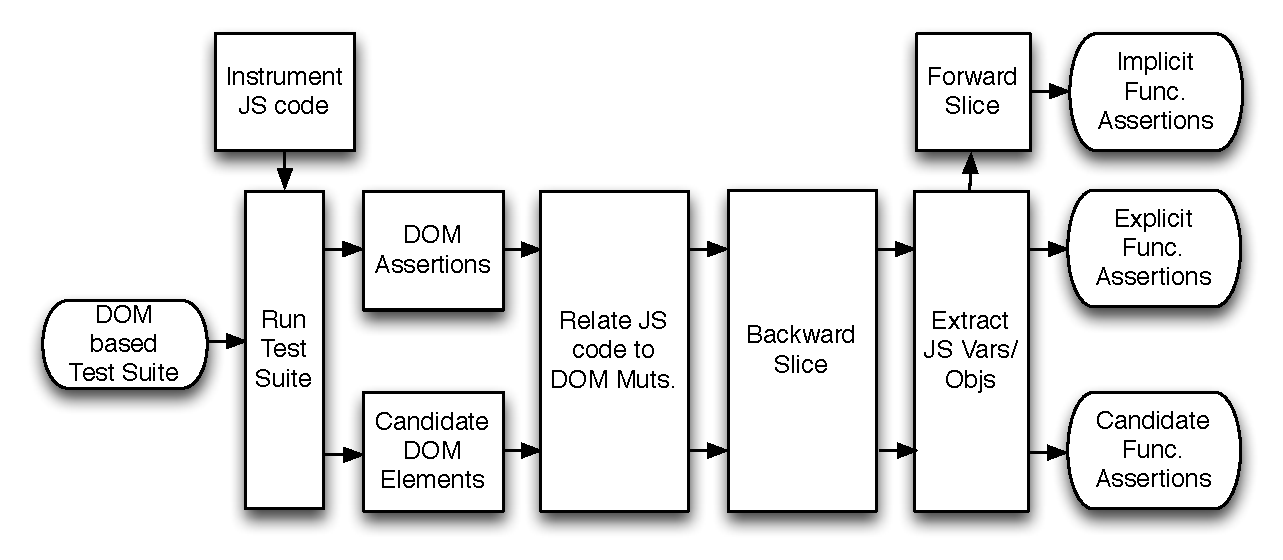
\includegraphics[width=.7\hsize]{fig/approachDiagram}
  \mycaption{Overview of our assertion generation approach.}
  \vspace{-0.1in} 
  \label{Fig:approachDiagram}
  \vspace{-0.1in} 
\end{figure*}
An overview of our \javascript function-level assertion generation technique is depicted in \figref{approachDiagram}.
At high level, our approach generates function level assertions for the \javascript code by utilizing human written DOM-based tests and assertions. Our code level assertions fall in the following three categories: (1) explicit assertions, which are directly inferred from analyzing the manually written DOM-based assertions, (2) implicit assertions, which are indirectly affected by the human written DOM-based assertions, and (3) candidate assertions, which are not considered in the written DOM-based assertions, yet are potentially useful to be checked by the function level test suite. We describe our approach below. The numbers below in parentheses correspond to those in the boxes of \figref{approachDiagram}.

In the first part of our approach we (1) instrument the \javascript code and execute the instrumented application by running the existing DOM-based test suite. In this step we gather a detailed execution trace of the application. We then extract (2) DOM-based assertions, and (3) candidate DOM element properties, which are useful DOM properties that can potentially be utilized for the purpose of assertion generation. We (4) identify the initial point of connection between the \javascript code and checked DOM element. We collect lines of code responsible for updating the corresponding DOM element. After determining DOM mutating statements, we (5) calculate the backward slice of these statements to find the entire code blocks that update the checked DOM element. We (6) extract \javascript entities including variables and objects associated with each of the obtained statements. Accessible entities form our explicit function level assertions (7). We further (8) perform a forward slice on the extracted \javascript entities to identify statements, that are implicitly affected by such entities. The accessible \javascript variables/objects associated with collected statements form our implicit function level assertions (9). In addition to explicit and implicit assertions, we also generate candidate assertions (10). Candidate assertions are involved with updating potentially useful DOM element properties, which are not checked in the existing DOM-based assertions. To obtain candidate function level assertions, we perform step (4), (5), and (6) on the inferred candidate DOM element properties (3).

Our overall unit-level assertion generation is presented in \algref{algorithm}. In the following sections we describe our technique for extracting DOM related information from the execution (\secref{extractDomRelatedInfo}), relating
DOM mutations to the \javascript code (\secref{domToCode}), and generating unit test assertions (\secref{unitLevelAssertion}).   
\subsection{Extracting DOM-Related Characteristics} \label{Sec:extractDomRelatedInfo}
The DOM connects a test case to the web application's code. Therefore, we first need to analyze the DOM-based test suite and extract the following pieces of information: (1) DOM-related operations of the existing test suite that may have tight connection with the \javascript code, and (2) frequently accessed DOM properties, which potentially are potentially influential in improving the fault finding capability of the test suite, but left unchecked in the manually-written test suite.
\headbf{DOM-Related Operations}
Any written test case needs to check the correctness of the application's behaviour. In a DOM-based test case the expected behaviour is checked through DOM-based assertions.
DOM-based assertion is defined as $<DOMProp,ExpVal>$, where $DOMProp$ is a DOM element feature (e.g. attribute, and/or textual value), and $ExpVal$ is the correct value expected by the assertion. Through the rest of the paper, we call DOM element feature as DOM property. 
DOM-based assertions play a significant role in our approach as they can guide us towards important portions of the underlying \javascript code that need to be checked in unit-level assertions.

For each DOM-based assertion we find \emph{Intra DOM assertion correlation} within the test suite.
\begin{mydef}[Intra DOM Assertion Correlation]
An intra DOM asseetion correlation is defined as a three tuple of $<DOMProp, AccDOM, AccDOMDep>$, where $DOMProp$ is the accessed DOM property within the assertion, $AccDOM$ is the accessed DOM elements in the test case pertaining to the assertion, and $AccDOMDep$ is the DOM dependencies of the assertion in the test case.
\end{mydef}
\textsc{GetDomAcc} in line 10 of \algref{algorithm} retrieves DOM dependencies of the assertion in the test case.
%, we instrument the test case by wrapping around method calls that accesses DOM elements.
Going back to our example in \figref{example}(b), tracking the assertion in line 11 shows that it has a DOM dependency to a \code{div} element with class \code{shopContainer}, which is accessed in line 10.

We further need to link the inferred Intra DOM assertion correlation with the application's code.
We call the correlation between the DOM-based assertion and the \javascript code of the application as \emph{inter DOM assertion correlation}.
\begin{mydef}[Inter DOM Assertion Correlation]
An inter DOM assertion correlation is defined as\\
$<AccDOMDep, InitCode>$, where $InitCode$ is the initial point of contact in the application's code segment, that is responsible for mutating $AccDOMDep$ the previously extracted DOM elements from the test suite.
\end{mydef}
To infer this type of correlation we track DOM's evolution of the $AccDOMDep$ (\textsc{GetDomMuts} in line 13 of the algorithm) as well as invoked event handlers as the test case runs. 
We consider additions and removals of child nodes, changes to attributes, and updates to child text nodes as DOM mutations. For instance, running the sample test case in \figref{example}(b) results in mutating (1) the textual value of \code{div} element with class \code{shopContainer}.
%We call the correlation between the DOM-based assertion and the \javascript code of the application as \emph{inter DOM assertion correlation}. This correlation is defined as $<AccDOMDep, InitCode>$, where $InitCode$ is the initial point of contact in the application's code segment, that is responsible for mutating the previously extracted DOM elements from the test suite ($AccDOMDep$).  
%We make use of \code{document.onload} event to log the initial DOM state. 
%An observer module is then used to monitor mutations on the DOM during the test case execution. 
%In addition to DOM changes, we also keep track of \javascript events as well as invoked event handlers. This information is later used to find the initial point of contact between a DOM mutation and the executed code segments.
%For instance, running the sample test case in \figref{example}(b) results in mutating (1) the textual value of \code{div} element with class \code{shopContainer}, and (2) the \code{class} attribute of DOM element with ID \code{couponButt}.
\headbf{Frequently Accessed DOM Properties}
In addition to DOM-based assertions, we further consider DOM element properties, that are frequently accessed within the application as the test case runs (lines 1 to 7 of \algref{algorithm}). 
\textsc{Acc} in line 6 of the algorithm computes the access frequency of a DOM property, $freqAccdDOM$ in line 7 contains the inferred candidate DOM properties, and \textsc{GetDomMuts} in line 19 records DOM mutations occur
on candidate DOM properties.
The intuition is that frequent use of a given DOM property can point to the extent of application's behaviour dependency on the DOM property. Thus, if changes happen to that property through the \javascript code, it is important to assert the correctness of such mutations. We define the access frequency of a DOM element property as the number of times that the element's property has been read during the execution of a test case. DOM properties include attributes as well as textual value of the elements.
In order to record DOM property accesses within the application, we rewrite native function calls used by programmers to access DOM element such as \code{getElementById}, \code{getElementsByClassName}, and/or \code{getElementsByTagName}. The returned object from these functions is later used to access attributes or textual values of the element. Thus, we apply a forward slice on the returned object to find instances of element's property access in the code.
For example in function \code{addToCart} of \figref{example}(a), DOM element with ID \code{couponButt} is assigned to \code{coupElem} variable. The assigned variable is later used to access the \code{class} attribute as well as the \code{value}
of the DOM element in lines 23, 25, and 26.

Let $Acc(prop_{el})$ be the access frequency computed for property $prop$ of DOM element $el$, then:
 
$Acc(prop_{el})=\frac{Read(prop_{el})}{\sum _{e=1}^{n} Read(domElem_e)}$, where $Read(domElem_{e})$ is the number of times that DOM element $domElem$ is read, given that the total number of DOM elements during the execution of a test case is $n$.
Note that reading a DOM element refers to accessing the element to read the corresponding property. In \figref{example}(a), the \code{class} attribute of DOM element \code{couponButt} is read in lines 23 and 34, and thus the access frequency
computed for the \code{class} attribute of the element is equal to $\frac{2}{3}$.

We choose element's property with access frequencies above a threshold $\alpha$ as potential candidates, which are later used for the purpose of unit-level assertion generation. We automatically compute this threshold for each test case as: 

$\alpha=\frac{1}{ReadProperties(T)}$, where $ReadProperties(T)$ is the total number of properties which have been read during the execution of test suite $T$.

Going back to our running example and the sample DOM-based test case in \figref{example}, \code{class} attribute of the \code{couponButt} is selected as a potential candidate since its access frequency ($\frac{2}{3}$) is greater than the computed threshold, which is equal to $\frac{1}{2}$ in this example.        
%application instrumentaion native event wrapping    

\subsection{Relating DOM Changes to the Code} \label{Sec:domToCode}
%\input{algorithm}
\begin{figure}[!t]
  \centering
  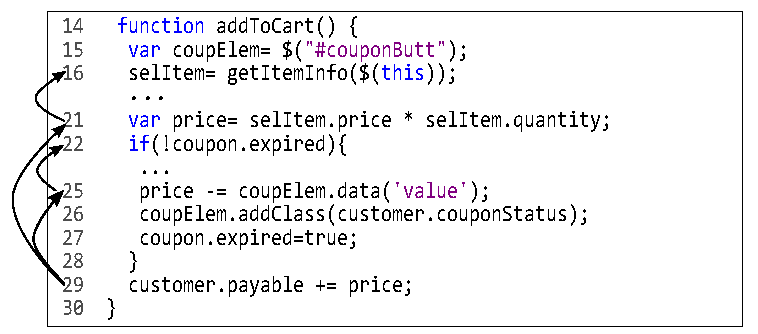
\includegraphics[width=1\hsize]{fig/intraCodeDep}
  \vspace{-0.3in} 
  \mycaption{Intra (data and control) code dependency through backward slicing.}
  \label{Fig:intraCodeDep}
  \vspace{-0.2in} 
\end{figure}
To determine the initial point of contact between DOM and the underlying application's code, we first cross reference the DOM element as well as the property we are interested in with a set of DOM mutations obtained from the execution trace. The desired DOM element and its property are inferred from either the intra DOM assertion dependency or the candidate DOM properties as described in \secref{extractDomRelatedInfo}. Recall that our execution trace contains information about triggered events, event handlers, and DOM mutations caused by the events. Therefore, we can identify relevant events and invoked functions corresponding to a given DOM mutation.
For example, the collected execution trace in \figref{assertionToCode} contains information about the mutations of a \code{div} element with class \code{shopContainer}, which pertains to the DOM-based assertion.

To figure out where the mutation originated in our execution trace, we keep record of DOM accesses within the invoked functions. For each DOM access, we track \javascript lines of code that are responsible for updating the corresponding DOM element. Going back to our example in \figref{assertionToCode}, given that the textual property of the \code{div} element is extracted from the intra DOM assertion dependency, we identify line 30 in function \code{viewCart} as the initial point of contact responsible for changing the \code{text} of DOM element.

After inferring DOM mutant statements, we identify the control and data \emph{intra code dependency} within the application's code.
%gather the entire set of \javascript statements responsible for mutating a given DOM element.
\begin{mydef}[Intra Code Dependency]
\label{def:intraCodeDep} 
 
An intra code dependency is defined as $<criterion, codeSts>$, where $criterion$ is a variable at the initial point of contact, and $codeSts$ is the set of control and data dependent statements that are either affected by the $ctiterion$ or have some effect on the $criterion$. 
\end{mydef}

To find the intra code dependency, we perform backward as well as forward slicing by using $criterion$ as the slicing criterion.
\textsc{GetBWSlice} in lines  15 and 21 of \algref{algorithm} computes a backward slice with respect to assertion related DOM mutations, and candidate DOM property mutations respectively.
We use dynamic slicing to capture run-time dependencies.
Note that instrumenting the entire application's code to perform dynamic slicing incurs high performance overheads. To avoid high overheads, we first intercept the code sent from the server to the client, and then statically instrument only those statements that may affect a given DOM element.
To extract the subset of the code statements, we first find the \javascript closure scope which contains the definition of the variable in the initial slicing criteria. Then all references to the variable within the closure scope are found. Therefore, we can identify all locations in the code where the variable is updated, read, or a new alias is created. For each variable update/read related to the variable of the slicing criteria, we track the data dependencies for such an operation. The aforementioned steps are performed iteratively for each dependencies to collect the subset of code statements, which are instrumented for a given initial slicing criteria.
The instrumented code keeps track of all updates and accesses to all relevant data and control dependencies.   
Once the test case runs, we collect traces from the instrumented code. This trace is used to dynamically extract backward slicing as well as forward slicing statements. Note that in addition to backwards slicing which is later used to generate explicit assertions, we also use forward slicing to generate our implicit assertions (\secref{implicitAssertions}).  

The backward slicing technique starts by extracting instances of the initial slicing criteria from the trace. For each \textit{read} operations, the trace is traversed backwards to find the nearest related \textit{write} operation. Once found, the \textit{write} operation is added to the slice under construction. This process is repeated for all the data dependencies related to that write operation. A similar approach is taken for including control dependencies in the slice. 
Our slicing technique supports inter-procedural slicing. For example, if a variable is assigned by the return value of a called function, the slicer recursively tracks the function and performs a backward slice on the statement returned by the called function.
%We track the following types of function calls during the slicing process: (1) Regular function calls e.g. \code{func()}, (2) Method calls e.g. \code{obj.func()}, (3) Constructors e.g. \code{new func()}, (4) Function handlers e.g. \code{element.click(func)}, and (5) Anonymous functions, which are assigned to a variable or an object property.
  
To address aliasing when computing the slice of a variable that has been set by a non-primitive value, we need to consider possible aliases that may refer to the same object. Specifically in \javascript \textit{dot notation} and \textit{bracket notation} are frequently used to modify objects at run time. Since static analysis techniques for \javascript often ignore this issue \cite{Feldthaus:icse13}, we use dynamic slicing. If a reference to an object of interest is saved to a second object's property, e.g. through the use of the \textit{dot notation}, the object of interest may also be altered via aliases of the second object. For example, after executing statement \code{a.b.c = objOfInterest;}, updates to \code{objOfInterest} may be possible through \code{a}, \code{a.b}, or \code{a.b.c}. To deal with such scenarios, our slicing technique searches through the collected trace and adds the forward slice for each detected alias to the current slice for our variable of interest (e.g. \code{objOfInterest}). 

Given \code{customer.payable} as the initial slicing criteria in our example, \figref{intraCodeDep} shows the relevant backward slice statements (lines 22, 18, 15, 14, and 9), where \code{customer.payable},  variable \code{price}, as well as properties of the object \code{selItem} are assigned, and the value of \code{coupon.expired} is checked in the conditional statement.
By the end of backward slicing step, we have all the relevant statements corresponding to a given DOM element. These are later used to derive test assertions.    
\subsection{Generating Unit-Level Assertions} \label{Sec:unitLevelAssertion}
Our approach targets postcondition assertions which are used to examine the expected behaviour of a given function after it is executed in a unit test case.
Through analyzing a given DOM-based test case, we generate unit-level assertions in the following three categories: (1) assertions, which are directly related to a given DOM-based assertion, (2) assertions, which are indirectly affected by a given DOM-based assertion, and (3) assertions that have direct impact on important DOM elements which are not checked by the existing DOM-based assertions. Each assertion is coupled with the expected value obtained from the execution trace of the application. The first type of assertion (type 1), which we call explicit assertion, can potentially be used in unit testing of the current version of the application. Type 2 and type 3, which we call implicit assertions and candidate assertions respectively, can be used for the purpose of regression testing.
\input{explicitAssertions}
\input{implicitAssertions}
\input{candidateAssertions}
          
%mutation of customer.couponStatus = coupon.Id + '-' + 'used' to customer.couponStatus = coupon.Id + 'used';'
\subsection{Tool Implementation: Atrina} \label{Sec:tool}

We have implemented our \javascript unit test assertion generation in an automated tool called \atrina. The tool is written in Java, and is publicly available for download \cite{atrina-dl}.
We use a proxy server to intercept HTTP responses which contain \javascript code. The \javascript Mutation Summary library \cite{mutationSummary} is used to track DOM changes during the execution of the test suite. Trace information is collected by the proxy once received from the browser. To instrument Selenium test cases, we convert them into an abstract syntax tree (AST) by employing Eclipse Java development tools (JDT). Once the transformation is done, we run the Java code of the changed AST on the application under test.   


\section{Empirical Evaluation} \label{Sec:evaluation}

To quantitatively assess the efficacy of our test generation approach, we have conducted an empirical study, in which we address the following research questions:

\begin{table*}
\centering
%\vspace{5pt}
        \caption{Characteristics of the experimental objects.}
{\scriptsize
    \begin{center}
       
      %  \subtable[Experimental subjects and the corresponding exploration data]
            {
           \begin{tabular}{c|l|c|c|c|l} \hline
\thead{App ID} &\thead{Name} &\thead{JS LOC} & \thead{\# Functions} &\thead{CC} &\thead{Resource}  \\  \hline \hline

1  & SameGame & 206 & 9 & 37 & \url{http://crawljax.com/same-game}   \\ \hline
           
2 & Tunnel & 334 & 32  & 39 & \url{http://arcade.christianmontoya.com/tunnel} \\ \hline

3 & GhostBusters & 277 & 27 & 52 & \url{http://10k.aneventapart.com/2/Uploads/657}  \\ \hline

4 & Symbol & 204 &  20 & 32  & \url{http://10k.aneventapart.com/2/Uploads/652}\\ \hline

5 & TuduList & 2767 &  229 & 28  & \url{http://tudu.ess.ch/tudu}\\ \hline

6 & SimpleCart (library) & 1702 & 23  &  168 & \url{http://simplecartjs.org}\\ \hline

7 & \jquery (library)& 8371  &  45 & 37  & \url{https://github.com/jquery/jquery}\\ \hline

8 & WymEditor & 3035  &  188 & 50  & \url{https://github.com/wymeditor}\\ \hline

\hline\end{tabular}\centering
            }
\label{Table:objectsChar-table}
\end{center}
}  
\vspace{-0.1in} 
\end{table*}

\begin{description}[noitemsep]
%\item [RQ1] How effective is our \emph{function coverage maximization} technique?
\item [RQ1] How effective is \tool in generating test cases with high coverage? 
\item [RQ2] How capable is \tool of generating test oracles that detect regression faults?
\item [RQ3] How does \tool compare to existing automated \javascript testing frameworks?
\end{description} 

%in which we compare \tool with an existing \javascript testing tool \artemis

\tool and all our experimental data produced are available for download \cite{jseft-dl}.



\subsection{Objects}
Our study includes thirteen \javascript-based applications in total. 
\tabref{objectsChar-table} presents each application's ID, name, lines of custom \javascript code (LOC, excluding \javascript libraries) and resource.
The first five are web-based games. AjaxTabs is a \jquery plugin for creating tabs. NarrowDesign and JointLondon are websites. FractalViewer is a fractal tree zoom application. SimpleCart is a  shopping cart library, WymEditor is a web-based HTML editor, Tudu\-List is a web-based task management application, and Tiny\-MCE is a \javascript based WYSIWYG editor control. The applications range from 206 to 27K lines of \javascript code.
%which has been used in other studies  \cite{artzi:icse11}. 

The experimental objects are open-source and cover different application types. All the applications are interactive in nature and extensively use \javascript on the client-side. %Since we require automated access and modification of the source code (\ie for instrumentation), we were not able to use applications such as FaceBook, where automated access is forbidden. %Moreover, since \tool does not support server-side testing, applications which their computations are mostly performed on the server side do not benefit from our approach.    


\subsection{Setup} \label{Sec:setup}
To address our research questions, we provide the URL of each  experimental object to \tool.
Test cases are then automatically generated by \tool.
%It is believed that \cite{humble:2010} testers dedicate no more than 10 minutes to test execution. Therefore, 
We give \tool 10 minutes in total for each application. 
5 minutes of the total time is designated for the dynamic exploration step.
%We outline the setup and methodology used in our empirical study to address our research questions.

%\subsubsection{Function Coverage Maximization (RQ1)}
%To measure the effectiveness of the function coverage maximization technique, we provide the URL of each experimental object to the first component of \tool as depicted in \figref{approach-view}. We compare our state/event selection strategy with a random exploration method, in which the next state is chosen uniformly at random for the expansion. 
%We limit the dynamic exploration time to five minutes \cite{humble:2010} for each technique and report the average results over five runs. We generate event sequences from the two state-flow graphs obtained from each method. 
%
%\jscover \cite{jscover}, an open-source tool for measuring \javascript code coverage, is used to measure the statement coverage. We collect the traces of the executed statements after each event is triggered. 
%Finally, we compare the statement coverage achieved by running the generated event sequences separately.
\headbf{Test Case Generation (RQ1)} \label{test-gen-setup}
To measure client-side code coverage, we use \jscover \cite{jscover}, an open-source tool for measuring \javascript code coverage. We report the average results over five runs.
In addition,  we assess each step in our approach separately as follows: 
(1) compare the statement coverage achieved by our function coverage maximization with a method that chooses the next state/event for the expansion uniformly at random, 
(2) assess the efficacy of our function state abstraction method (\algref{stateAbstractionAlgo}), and 
(3) evaluate the effectiveness of applying mutation techniques (\algref{oracleGenAlgo}) to reduce the number of assertions generated.
% we provide the URL of each experimental object to the first component of \tool as depicted in \figref{approach-view}. We compare our state/event selection strategy with a random exploration method, in which the next state is chosen uniformly at random for the expansion. 
%We generate event sequences from the two state-flow graphs obtained from each method. 

%We collect the traces of the executed statements after each event is triggered. 
%Finally, we compare the statement coverage achieved by running the generated event sequences separately. 

%Of course, no unit test generation technique can test functions that are not directly accessible (\eg nested functions, anonymous functions).
%Therefore, in addition to measuring the statement coverage of the generated test suite, we define a unit testability metric, which measures the testability degree of individual functions of an application. We call a function $f$ \emph{testable} if it is possible to call $f$ directly from a test case --- regardless of whether the test case is written manually or generated automatically. The testability metric of a given web application $A$ is calculated as follows: 
%
%\begin{equation}
%testability(A)=\frac{\sum _{i\in A(f_i)}^{n} {testable(f_i)}}{n},
%\label{testabilityFormula}
%\end{equation}
%\noindent
%where $n$ is the total number of functions, and $testable$ decides whether a function ($f_i$) is testable according to the definition. We then measure the percentage of functions that \tool can generate test cases for in $A$ as:   
%
%\begin{equation}
%testGenRate(A)=\frac{\sum _{i\in A(f_i)}^{n} {tested(f_i)}}{\sum _{i\in A(f_i)}^{n} {testable(f_i)}},
%\label{pythiaTestabilityFormula}
%\end{equation}
%\noindent
%where the numerator is the total number of functions that are directly tested by \tool and the denominator is the total number of testable functions in $A$.

\headbf{Test Oracles (RQ2)} \label{test-oracle-setup}
%To generate test oracles at function-level, we configure \tool to inject 50 \javascript code-level faults in each application.
%To produce DOM event-level oracles, we configure the DOM mutation module of \tool to inject 20 DOM-level faults per application. \ali{why 50? why 20? why these numbers? why are they not the same? Motivate! Do we need to include this information?} %We then run \tool on each web application to obtain the test cases with oracles.
%
To evaluate the fault finding capability of \tool (RQ2), we simulate web application faults by automatically seeding each application with 50 random faults. %according to the following fault category: 
%\begin{enumerate}[noitemsep, nolistsep]
%\item Changing conditional statements by modifying the upper/lower bounds of loop statements, 
%changing the condition itself, as well as swapping consecutive conditional statements;
%\item Modifying the values of global/local variables, and removing or changing their names, as well as modifying arithmetic operations;
%\item Changing function parameters or function call arguments by swapping, removing,
%and renaming parameters/arguments. Changing the sequence of function
%calls within a given function if applicable;
%\item Modifying DOM related properties.
%\end{enumerate}
%The first three categories target \javascript code while the last one targets both \javascript and HTML code-levels. 
We automatically pick a random program point and seed a fault at that point according to our fault category.
While mutations used for oracle generation have been selectively generated (as discussed in \secref{oracleGen}), 
mutations used for the purpose of evaluation are randomly generated from the entire application. Note that if the mutation used for the purpose of evaluation and the mutation used for generating oracles happen to be the same, we remove the mutant from the evaluation set. 
%in the \javascript code as well as the HTML code of each application. 
%Note that we decided to manually perform fault seeding instead of using \mutandis, which automates \javascript mutation testing. The main reason is to mitigate bias since \mutandis is used by \tool to generate mutants automatically during the test oracle generation phase. 
%One challenge with generating assertions is their stability, \ie the assertions may fail on the original version of the program. To filter unstable assertions, we run the test suite on the original program and discard any assertions that fail.
%
Next we run the whole generated test suite (including both function-level and event-based test cases) on the faulty version of the application. The fault is considered detected if an assertion generated by \tool fails and our manual examination confirms that the failed assertion is detecting the seeded fault.
%\ali{how do we know we have detected the right fault?}
We measure the precision and recall as follows:

\begin{description}[noitemsep, nolistsep]
\item[Precision] is the rate of injected faults found by the tool that are actual faults: $\frac{\mathit{TP}}{\mathit{TP} + \mathit{FP}}$
\item[Recall] is the rate of actual injected faults that the tool finds: $\frac{\mathit{TP}}{\mathit{TP} + \mathit{FN}}$ 
\end{description}
where $\textit{TP}$ (true positives), $\textit{FP}$ (false positives), and $\textit{FN}$ (false negatives) respectively represent the number of faults that are correctly detected, falsely reported, and missed.

\headbf{Comparison (RQ3)} \label{comparison-setup}
To assess how \tool performs with respect to existing \javascript test automation tools, we compare its coverage and fault finding capability to that of \artemis \cite{artzi:icse11}.  
Similar to \tool, we give \artemis 10 minutes in total for each application; we observed no improvements in the results obtained from running \artemis for longer periods of time. 
We run \artemis from the command line by setting the iteration option to 100 and enabling the coverage priority strategy, as described in \cite{artzi:icse11}. %\karthik{Earlier you said 5 minutes}. 
Similarly, JSCover is used to measure the coverage of \artemis (over 5 runs).
We use the output provided by \artemis to determine if the seeded mutations are detected by the tool, by following the same procedure as described above for \tool. 
%We measure the coverage using the HTML output of \artemis, which shows the covered \javascript code. %As mentioned before, we measure the coverage of \tool using \blanket.


\subsection{Results} \label{Sec:results}

%\input{covg-table} 


%\headbf{Function coverage maximization (RQ1)} \tabref{efficiency-abs-mut-table} presents the statement coverage achieved by using our function coverage maximization technique and the random strategy. Our results show on average 9\% improvement in statement coverage, across all the applications. We observed that our technique achieves the highest improvement when there are dynamically generated clickables in the application.
%
%For example, for Tunnel (ID 2) and Fractal Viewer (ID 9), we observed no improvement in the statement coverage as these two applications have no dynamically generated or bound to event-listeners clickables. Instead, their few clickables are all placed in the HTML code of the application with a fixed event-handler per clikcable. Thus,  our approach achieves the same coverage as the random strategy for such applications.
%
%For SameGame (ID 1) the number of executed functions remains the same, for both approaches. However, in the limited five minute period of time, as a result of dynamically detecting valid clickable elements, \tool is able to examine different paths of the applications, while the random exploration technique fails to do so as it blindly clicks on any candidate element on the DOM tree.
%
%Finally, GhostBusters (ID 3) benefits the most from our dynamic exploration technique. This application contains a large number of dynamically created clickable DOM elements that appear and then disappear within a few seconds. We observed two anonymous functions, attached to clickable elements, that are missed by the random exploration technique in this application. Our technique is not only able to quickly spot such on the fly generated clickables, but it is also able to click on the ones that result in the execution of uncovered functions. 
%These two functions are attached to clickable elements that are not executed using random strategy. 

\input{efficiency-abs-mut-table}

\begin{figure}[!t]
  \centering
  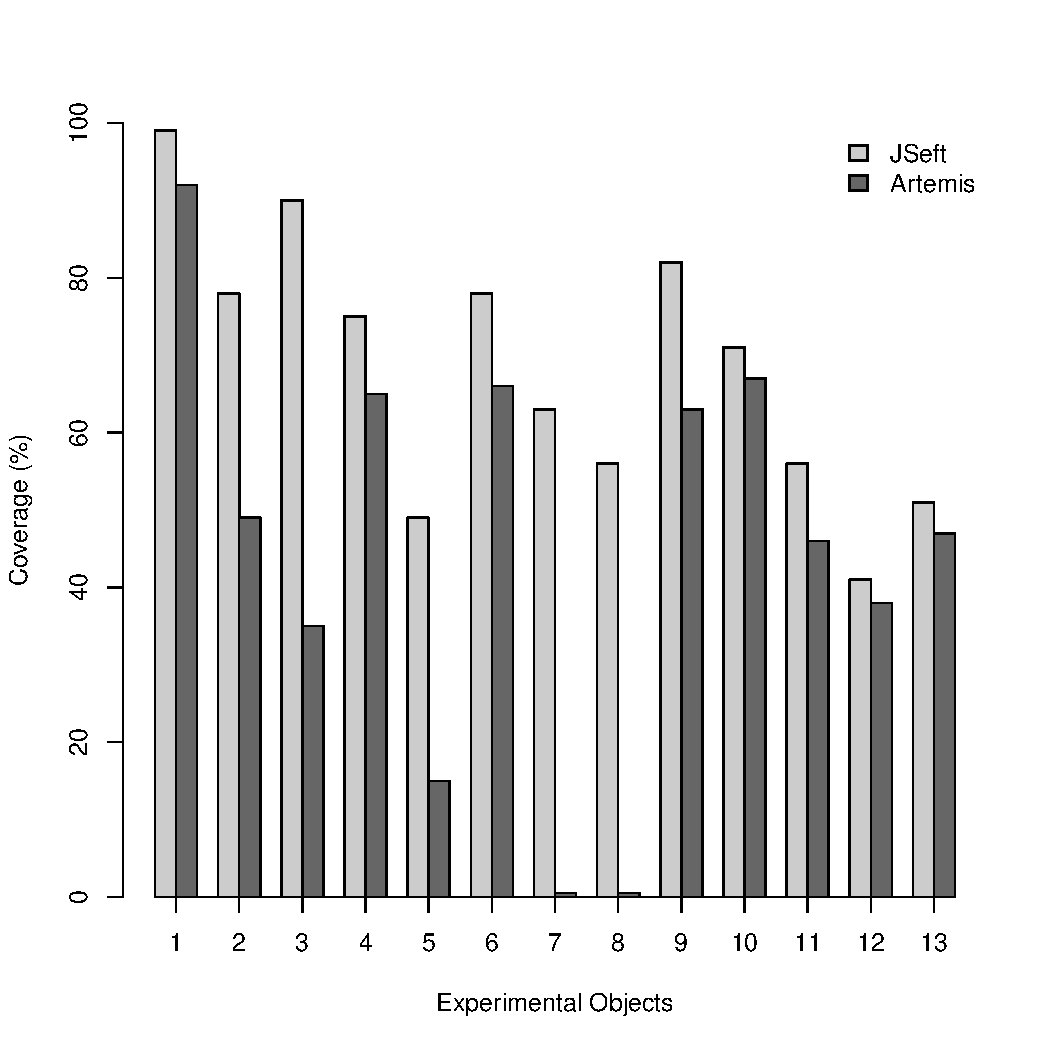
\includegraphics[width=1\hsize]{r-scripts/barplot_coverage}
  \vspace{-0.1in} 
  \mycaption{Statement coverage achieved.} 
  \vspace{-0.25in} 
  \label{Fig:coverage-graph}
\end{figure}


\headbf{Test Case Generation (RQ1)} 
\figref{coverage-graph} depicts the statement coverage achieved by \tool for each application. The results show that the test cases generated by \tool achieve a coverage of 68.4\% on average, ranging from 41\% (ID 12) up to 99\% (ID 1).
%\karthik{Do we need the text below ? We are better than random.}
We investigated why \tool has low coverage for some of the applications. For instance, we observed that in JointLondon (ID 7), the application contains \javascript functions that are browser/device specific, i.e., they are exclusively executed in Internet Explorer, or iDevices. As a result, we are unable to cover them using \tool. 
We also noticed that some applications required more time to achieve higher statement coverage (e.g., in NarrowDesign ID 8), or they have a large DOM state space (e.g., BunnyHunt ID 5) and hence \tool is only able to cover a portion of these applications in the limited time it had available.

\tabref{efficiency-abs-mut-table} columns under ``St. Coverage'' present \javascript statement coverage achieved by  our function coverage maximization algorithm versus a random strategy. The results show a 9\% improvement on average, for our algorithm, across all the applications. We observed that our technique achieves the highest improvement when there are many dynamically generated clickable DOM elements in the application, for example, GhostBusters (ID 3). 
%For instance, GhostBusters (ID 3) has 27\% more coverage since it contains a large number of dynamically created clickable DOM elements that appear and then disappear within a few seconds, which our technique can handle, but the random one may not. 
%We observed two anonymous functions, attached to clickable elements, that are missed by the random exploration technique in this application. Our technique is not only able to quickly spot such on the fly generated clickables, but it is also able to click on the ones that result in the execution of uncovered functions.

The columns under ``State Abstract'' in \tabref{efficiency-abs-mut-table} present the number of function states
before and after applying our function state abstraction algorithm.   
The results show that the abstraction strategy reduces function states by 85.5\% on average. NarrowDesign (ID 7) and FractalViewer (ID 9) benefit the most by a 97\% state reduction rate. 
%\karthik{What about ID 9 ?}
Note that despite this huge reduction, our state abstraction does not adversely influence the coverage as we include at least one function state from each of the covered branch sets as described in \secref{testCaseGen}.

The last two columns of \tabref{efficiency-abs-mut-table}, under ``Oracles'', present the number of assertions obtained by capturing the whole application's state,  without any mutations, and with our mutation-based oracle generation algorithm respectively. The results show that the number of assertions is decreased by 86.5\% on average due to 
our algorithm. 
We observe the most significant reduction of assertions for JointLondon (ID 7) from more than 198000 to 342. 
%\ali{by how much? what is the reduction rate?} 


%\ali{removing the insiginificant results} For example, for Tunnel (ID 2) and Fractal Viewer (ID 9), we observed no improvement in the statement coverage as these two applications have no dynamically generated or bound to event-listeners clickables. Instead, their few clickables are all placed in the HTML code of the application with a fixed event-handler per clikcable. Thus,  our approach achieves the same coverage as the random strategy for such applications.
%For SameGame (ID 1) the number of executed functions remains the same, for both approaches. However, in the limited five minute period of time, as a result of dynamically detecting valid clickable elements, \tool is able to examine different paths of the applications, while the random exploration technique fails to do so as it blindly clicks on any candidate element on the DOM tree.



%These two functions are attached to clickable elements that are not executed using random strategy.
%\figref{coverage-graph} presents our results for the statement coverage achieved by the test suite generated by \tool and \artemis. %The coverage is shown separately for the function-level unit tests and DOM event-based tests.     
%\tabref{efficiency-abs-mut-table} presents the number of function states
%before and after applying our function state abstraction mechanism.    
%The results show that the abstraction strategy is able to reduce the number of function states up to 97\%. NarrowDesign (id 7) with the largest
%number of function states benefits the most from our abstraction technique by 97\% state reduction. Note that we observed that our state abstraction does not affect the coverage. The reason is we select at least one function state from each of the covered branch sets as described in \secref{testCaseGen}.
%The last two columns of \tabref{efficiency-abs-mut-table} presents the number of all possible assertions obtained by capturing the whole application's state without performing any mutation, as well as the number of assertions after applying mutation. The results show that the number of assertions are drastically reduced by selectively pick only useful assertions during the mutation process.
% \tabref{testability-table} presents the testability of \javascript functions in the experimental objects.
% The table shows the total number of functions, number of functions that are testable, and the percentage of testable functions. 
% It also shows the number and the percentage of testable functions that are tested by the function-level tests generated by \tool (See Definitions \ref{testabilityFormula}-\ref{pythiaTestabilityFormula} in Section \ref{test-gen-setup}). 
% 
%As shown in \tabref{testability-table}, our generated function-level unit tests can, on average, examine 77\% of the testable functions. 
%This demonstrates the efficacy of our function covering technique in covering a considerable number of functions. 
%While \tool is able to examine up to 100\% of the testable functions for  SameGame, it can only cover 48\% of the testable functions for Fractal Viewer. 
%The low numbers for Fractal Viewer are mainly due to (1) the presence of random generator functions, and (2) the lack of support  for object input parameters with cyclic references in the current implementation of \tool, which we discuss in \secref{discussion}.

\input{faultDetection-table}
\headbf{Fault finding capability (RQ2)} \tabref{faultDetection-table} presents the results on the fault finding capabilities of \tool.
The table shows the total number of injected faults, the number of false negatives, false positives, true positives, and the precision and recall of \tool. 

\tool achieves 100\% precision, meaning that all the detected faults reported by \tool are real faults. {\em In other words, there are no false-positives.}
This is because the assertions generated by \tool are all stable \ie they do not change from one run to another. % as we do not observe any false positives. 
However, the recall of \tool is 70\% on average, and ranges from 48 to 100\%. This is due to false negatives, \ie missed faults by \tool, 
which occur when the injected fault falls is either in the uncovered region of the application, or is not properly captured by the generated oracles.  

%\begin{figure}[!t]
%  \centering
%  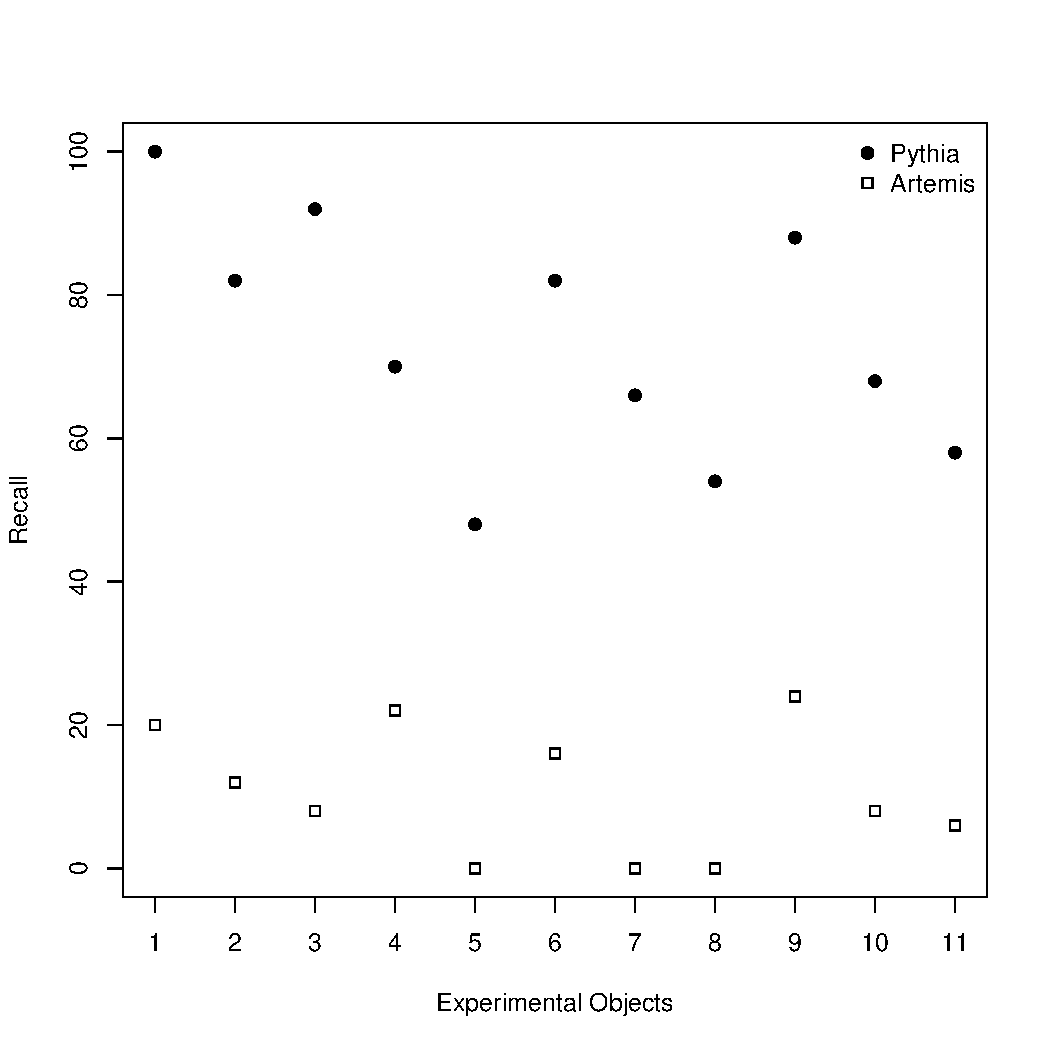
\includegraphics[width=0.9\hsize]{r-scripts/recall}
%  \mycaption{Recall of \tool and \artemis in detecting faults.}
%  \vspace{-0.1in} 
%  \label{Fig:recall-graph}
%\end{figure}

The table also shows that on average 32\% percent of the injected faults (ranges from 15--73\%) are detected by function-level test cases, but not by our DOM event-based test cases. This shows that a considerable number of faults do not propagate to observable DOM states, and thus cannot be captured by DOM-level event-based tests. 
For example in SimpleCart application (ID 10), if we mutate the mathematical operation that is responsible for computing the total amount of purchased items, the resulting error is not captured by event-based tests as the fault involves internal computations only. However, the fault is detected by a function-level test that directly checks the returned value of the function.
This points to the importance of incorporating function-level tests in addition to event-based tests for \javascript web applications. We also observed that even when an event-based test case detects a \javascript fault, localizing the error to the corresponding \javascript code can be quite challenging. However, function-level tests pinpoint the  corresponding function when an assertion fails, making it easier to localize the fault. 
%For example, in SameGame (ID 1), the function \code{compactDown} is responsible for moving cells up on the board after clicking on a given cell. If the index of the global variable \code{board} array is mutated in \code{compactDown}, the event-based tests shows an incorrect \code{background} value of the \code{css} property on the corresponding DOM elements. However, tracing the fault back to the responsible function is difficult. Using function-level tests, we can easily spot the assertion that is failed after calling \code{compactDown} function (e.g., \code{equal(board[3][4], 1)} failed).    

\headbf{Comparison (RQ3)}
\figref{coverage-graph} shows the code coverage achieved by  both \tool and \artemis on the experimental objects running for the same amount of time, \ie 10 minutes.
%Note that while \artemis only generates DOM event tests, \tool generates both unit tests and DOM event tests. 
%We compare the statement coverage achieved by \tool with that achieved by \artemis. 
The test cases generated by \tool achieve 68.4\% coverage on average (ranging from 41--99\%), while \artemis achieves only 44.8\% coverage on average (ranging from 0--92\%).
Overall, the test cases generated by \tool achieve 53\% more coverage than \artemis, which points to the effectiveness of \tool in generating high coverage test cases. 
Further, as can be seen in the bar plot of \figref{coverage-graph}, for all the applications, the test cases generated by \tool achieve higher coverage than those generated by \artemis. 
This increase was more than 226\% in the case of Bunnyhunt (ID 5). %\ali{Is this true? Isn't the difference in ID 7 and ID 8 more?}
For two of the applications, NarrowDesign (ID 7) and JointLondon (id 8), \artemis was not able to complete the testing task within the allocated time of ten minutes.
Thus we let \artemis run for an extra 10 minutes for these applications (\ie 20 minutes in total). Even then, neither application completes under \artemis. 
%By reducing the iteration option, \artemis produces an output after 10 minutes, however, with considerably lower coverage rates of 30\% and 35\% for NarrowDesign (ID 7), and JointLondon (ID  8), respectively. %I calculated the results based on zero coverage for these two apps, not sure if mentioning 30 and 35% here is correct or not!   

\tabref{faultDetection-table} shows the precision and recall achieved by \tool and \artemis.
With respect to fault finding capability, unlike \artemis that detects only generic faults such as runtime exceptions and W3C HTML validation errors, \tool is able to accurately distinguish faults at the code-level and DOM-level through the test oracles it generates. Both tools achieve 100\% precision, however, \tool achieves five-fold higher recall (70\% on average) compared with \artemis, which achieves 12.8\% recall on average. %Thus, \tool achieves more than five-fold increase in recall over \artemis.   

\subsection{Threats to Validity} \label{Sec:threatsToValidity}
An external threat to the validity of our evaluation is the limited number of \javascript applications used to measure the effectiveness of our approach. We mitigated this threat by using web applications from various domains, code size, and functionality. Another threat concerns validating failed assertions through manual inspection that can be error-prone. To mitigate this threat, we carefully examine the code in which the assertion failed to make sure that the injected fault was indeed responsible for the assertion failure. Moreover, manual computation of the \javascript slices to measure precision and recall is a time intensive task done by the authors of the paper, and thus could be error-prone. However, we made every effort to mitigate this threat by precisely examining the application's code.

The regression faults we inject to evaluate the effectiveness of \tool may not be realistic. We mitigate this threat by injecting mutations that represent common \javascript applications faults, as well as using real-world web applications, and \selenium test cases written by developers.
%\subsection{Discussion} \label{Sec:discussion}
\begin{figure}[!t]
  \centering
  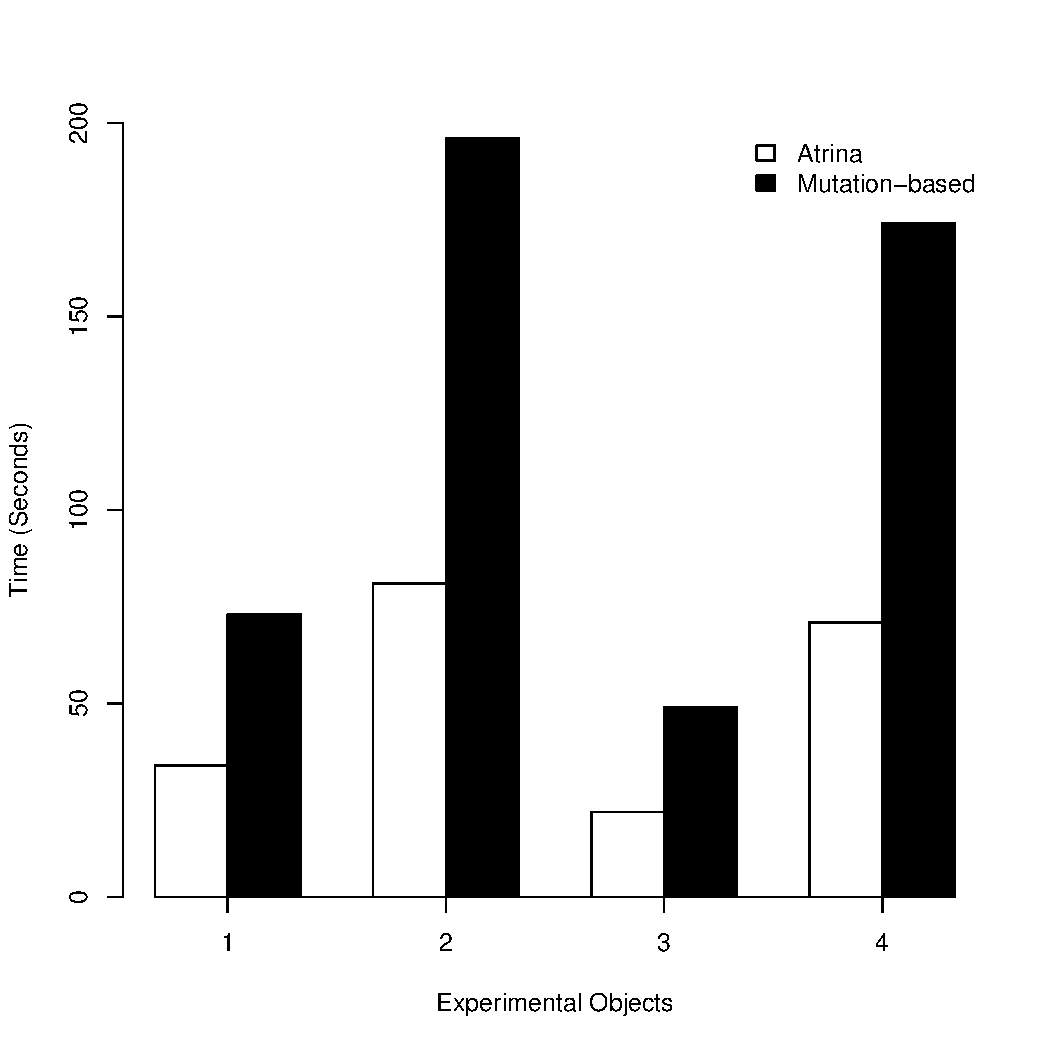
\includegraphics[width=0.7\hsize]{r-scripts/performance}
  \vspace{-0.18in}   
  \mycaption{Time overhead for each approach.}
  \vspace{-0.3in} 
  \label{Fig:performance}   
\end{figure}
% Moved time efficiency to results
%Moreover, this reiterates the known performance shortcomings of approaches that rely on mutant generation.
\headbf{Fault Masking} As we mentioned in \secref{explicitAssertions}, the concrete value of an entity in the computed backward slice can potentially be used as the expected value of the entity in explicit assertions to test the current version of the application.
The actual values of the related entities in the backward slice are correct unless there exists a masked fault which is concealed in the chain of computations and thus does not propagate to the checked state of the DOM element. However, we conjecture that fault masking rarely happens in \javascript web applications as it is more prevalent in programs with many small expressions whose results are stored in several intermediate values. We also observed no fault masking occurrence during the evaluation of \tool on seven \javascript applications used in this study.
\headbf{Limitations} The effectiveness of the generated assertions by \tool in terms of fault finding capability depends on the quality of human-written DOM-based test cases. If the DOM assertions contained in the DOM-based test suite check irrelevant information, the explicit assertions obtained by our tool will point to entities that may not be important from the tester's point of view. This can also negatively affect the fault finding capability of implicit assertions as they are indirectly inferred from the DOM-based assertions. Moreover, if the human-written test suite does not execute application's state with effective DOM elements, our tool is not able to infer effective candidate assertions.   


  

\subsection{Discussion} \label{Sec:discussion}
\begin{figure}[!t]
  \centering
  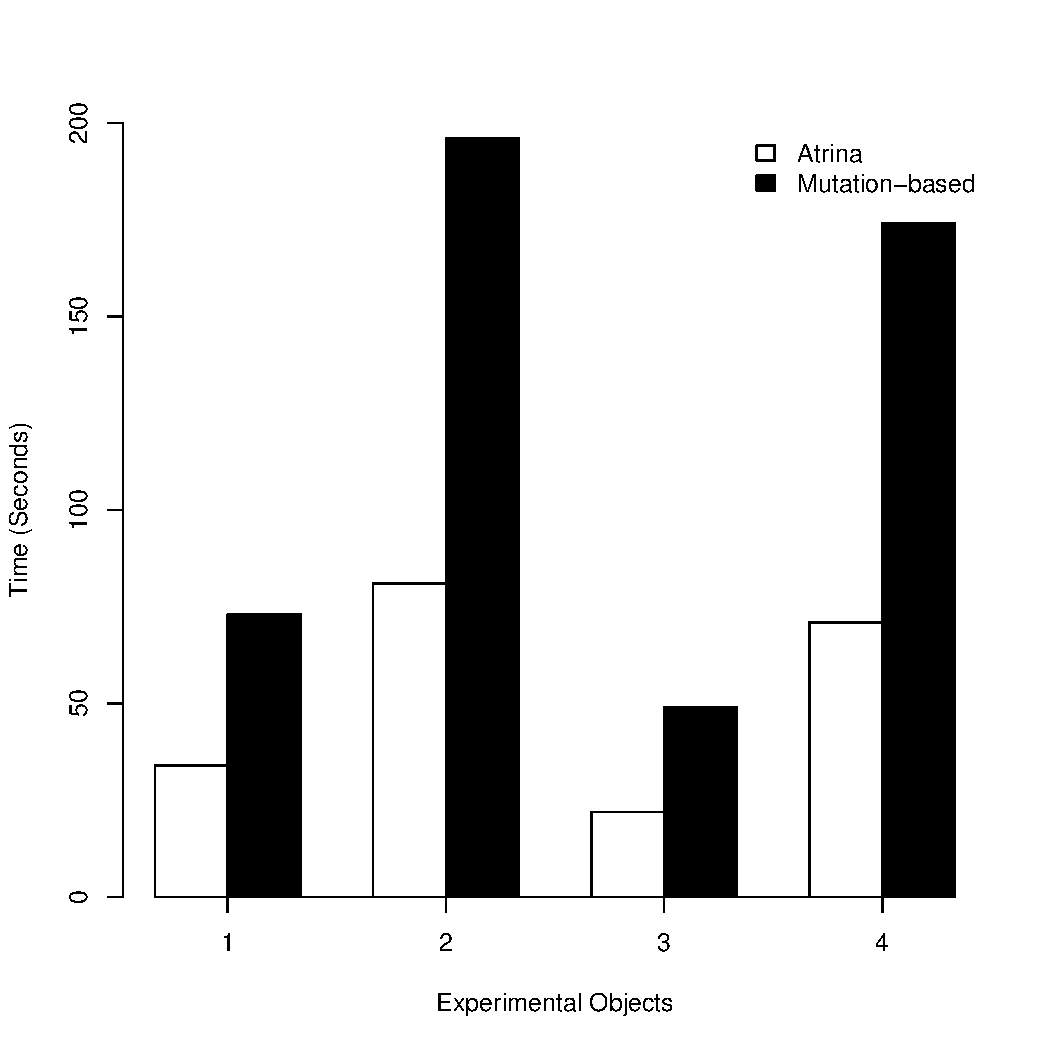
\includegraphics[width=0.7\hsize]{r-scripts/performance}
  \vspace{-0.18in}   
  \mycaption{Time overhead for each approach.}
  \vspace{-0.3in} 
  \label{Fig:performance}   
\end{figure}
% Moved time efficiency to results
%Moreover, this reiterates the known performance shortcomings of approaches that rely on mutant generation.
\headbf{Fault Masking} As we mentioned in \secref{explicitAssertions}, the concrete value of an entity in the computed backward slice can potentially be used as the expected value of the entity in explicit assertions to test the current version of the application.
The actual values of the related entities in the backward slice are correct unless there exists a masked fault which is concealed in the chain of computations and thus does not propagate to the checked state of the DOM element. However, we conjecture that fault masking rarely happens in \javascript web applications as it is more prevalent in programs with many small expressions whose results are stored in several intermediate values. We also observed no fault masking occurrence during the evaluation of \tool on seven \javascript applications used in this study.
\headbf{Limitations} The effectiveness of the generated assertions by \tool in terms of fault finding capability depends on the quality of human-written DOM-based test cases. If the DOM assertions contained in the DOM-based test suite check irrelevant information, the explicit assertions obtained by our tool will point to entities that may not be important from the tester's point of view. This can also negatively affect the fault finding capability of implicit assertions as they are indirectly inferred from the DOM-based assertions. Moreover, if the human-written test suite does not execute application's state with effective DOM elements, our tool is not able to infer effective candidate assertions.   
%\section{Related Work}
\label{Sec:relatedWork}

Automated testing of modern web applications is becoming an active area of research \cite{artzi:icse11,tonella:icst08,mesbah:tse12,dodom:2010}.
Most of the existing work on \javascript analysis is, however, focused on spotting errors and security vulnerabilities through static analysis \cite{Guarnieri-2009,Guha-2009,Zheng-2011}.
We classify related work into two broad categories: web application regression testing and program invariants.

%\begin{description}
%\item[JavaScript Analysis]
%\head{JavaScript Analysis.}
%Automated testing of modern web applications is becoming an active area of research \cite{artzi:icse2011,tonella:icst08,mesbah:tse12,dodom:2010}.
%Most of the existing work on \javascript analysis is, however, focused on spotting errors and security vulnerabilities through static analysis \cite{Guarnieri-2009,Guha-2009,Zheng-2011}.
%Kudzu \cite{song:symb10} is a symbolic execution system for \javascript aimed at automated security vulnerability analysis. %This is done by automatically generating a test suite using symbolic execution of the \javascript source code. 
%BrowserShield \cite{reis:tweb} applies 
%dynamic instrumentation to rewrite \javascript code to conduct vulnerability driven filtering. Yu \etal \cite{yu:javascript} propose a method in which untrusted \javascript code is analyzed and instrumented \cite{Kikuchi08javascript} to identify and modify questionable behaviour.


\head{Web Application Regression Testing.}
Regression testing of web applications has received relatively limited attention from the research community \cite{lei:reg03,tarhini:reg08}.
Alshahwan and Harman~\cite{harman:icst08} discuss an algorithm for regression testing of web applications that is based on session data \cite{sprenkle:replayweb,elbaum:webtest} repair. Roest et al. \cite{Roest:2010.icst} propose a technique to cope with the dynamism in Ajax web interfaces while conducting automated regression testing. None of these works, however, target regression testing of \javascript in particular.

\head{Program Invariants.}
The concept of using invariants to assert program behaviour at runtime is as old as programming itself \cite{Clarke:2006}. A more recent development is the automatic detection of program invariants through dynamic analysis. Ernst \etal have developed Daikon \cite{ernst2007daikon}, a tool capable of inferring likely invariants from program execution traces. Other related tools for detecting invariants include Agitator \cite{agitator:issta06}, DIDUCE \cite{Hangal02trackingdown}, and DySy \cite{Csallner08dysy}. Recently, Ratcliff \etal \cite{ratcliff:gecco11} have proposed a technique to reuse the trace generation of Daikon and integrate it with genetic programming to produce useful invariants.  %DySy is somewhat different than the rest, since it is based on an algorithm that uses symbolic execution of the program as well as its concrete execution to detect likely invariants. Swaddler \cite{CovaBFV2007} is an invariant detection tool for PHP that is based on Daikon.
Conceptually related to our work, Rodr{\'\i}guez-Carbonell and Kapur \cite{rodrikapurICTAC04} use  inferred invariant assertions for program verification.

Mesbah \etal \cite{mesbah:tse12} proposed a framework called \atusa for manually specifying generic and application-specific invariants on the DOM-tree and \javascript code. These invariants were subsequently used as test oracles to detect erroneous behaviours in modern web applications. Pattabiraman and Zorn proposed DoDOM \cite{dodom:2010}, a tool for inferring invariants from the DOM tree of web applications for reliability testing.

To the best of our knowledge, this work is the first to propose an automated regression testing approach for \javascript, which is based on  \javascript invariant assertion generation and runtime checking.



%\chapter{Conclusion} \label{Chap:conc}
\javascript is increasingly being used to create modern interactive web applications that offload a considerable amount of their execution to the client-side. \javascript is a notoriously challenging language for web developers to use, maintain, analyze and test. This thesis has focused on exploring strategies for testing \javascript-based web applications. In accordance to the goal of this dissertation we designed two research questions:
\begin{itemize}
\item [RQ1] How can we generate effective test cases for \javascript web applications?
\item [RQ2] How can we effectively assess the quality of the written test suites for \javascript applications?
\end{itemize}
\section{Contributions}
%The main contributions of the thesis can be summarized as follows:
The main contributions of the thesis in response to the first research question (RQ1) are as follows: 
\begin{itemize}
\item A new automated technique for \javascript regression testing, which is based on dynamic analysis to infer invariant assertions; The obtained assertions are injected back into the \javascript code to uncover regression faults in subsequent revisions of the web application under test. 
\item An automatic technique to generate test cases for \javascript functions and events; We use a mutation-based algorithm to effectively generate test oracles, capable of detecting regression \javascript and DOM-level faults. The technique uses a combination of function converge maximization and function state abstraction algorithms to efficiently generate unit test cases.
\item Exploiting an existing DOM-based test suite to generate unit-level assertions for applications that highly interact with the DOM through the underlying \javascript code; We utilize
existing DOM-dependent assertions as well as useful execution information inferred from a DOM-based test suite to automatically generate assertions used for testing individual \javascript functions.
\end{itemize}
To address the second research question (RQ2), we made the following contribution:
\begin{itemize}
\item The first \javascript mutation testing tool, which is capable of guiding the mutation generation towards behaviour-affecting mutants in error-prone portions of the code; The mutation testing method combines dynamic and static analysis to mutate branches that are within highly ranked functions and exhibit high structural complexity.
\end{itemize}

%    2. Main body
% Generally recommended to put each chapter into a separate file
%\include{relatedwork}
%\include{model}
%\include{impl}
%\subsection{Discussion} \label{Sec:discussion}
\begin{figure}[!t]
  \centering
  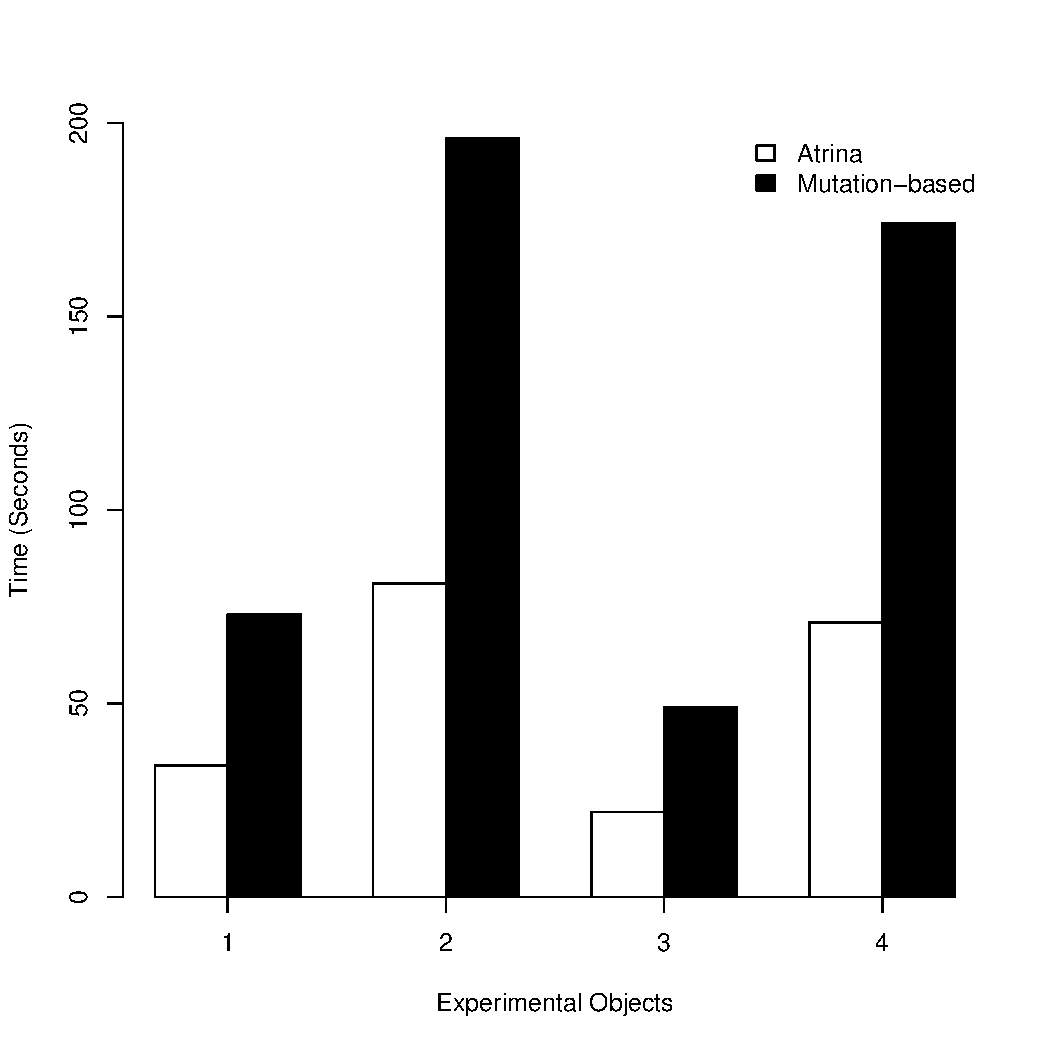
\includegraphics[width=0.7\hsize]{r-scripts/performance}
  \vspace{-0.18in}   
  \mycaption{Time overhead for each approach.}
  \vspace{-0.3in} 
  \label{Fig:performance}   
\end{figure}
% Moved time efficiency to results
%Moreover, this reiterates the known performance shortcomings of approaches that rely on mutant generation.
\headbf{Fault Masking} As we mentioned in \secref{explicitAssertions}, the concrete value of an entity in the computed backward slice can potentially be used as the expected value of the entity in explicit assertions to test the current version of the application.
The actual values of the related entities in the backward slice are correct unless there exists a masked fault which is concealed in the chain of computations and thus does not propagate to the checked state of the DOM element. However, we conjecture that fault masking rarely happens in \javascript web applications as it is more prevalent in programs with many small expressions whose results are stored in several intermediate values. We also observed no fault masking occurrence during the evaluation of \tool on seven \javascript applications used in this study.
\headbf{Limitations} The effectiveness of the generated assertions by \tool in terms of fault finding capability depends on the quality of human-written DOM-based test cases. If the DOM assertions contained in the DOM-based test suite check irrelevant information, the explicit assertions obtained by our tool will point to entities that may not be important from the tester's point of view. This can also negatively affect the fault finding capability of implicit assertions as they are indirectly inferred from the DOM-based assertions. Moreover, if the human-written test suite does not execute application's state with effective DOM elements, our tool is not able to infer effective candidate assertions.   
%\include{conclusions}

%    3. Notes
%    4. Footnotes

%    5. Bibliography
\begin{singlespace}
\raggedright
\bibliographystyle{abbrvnat}
\bibliography{../biblio}
\end{singlespace}

\appendix
%    6. Appendices (including copies of all required UBC Research
%       Ethics Board's Certificates of Approval)
%\include{reb-coa}	% pdfpages is useful here
\chapter{Supporting Materials}

This would be any supporting material not central to the dissertation.
For example:
\begin{itemize}
\item additional details of methodology and/or data;
\item diagrams of specialized equipment developed.;
\item copies of questionnaires and survey instruments.
\end{itemize}


\backmatter
%    7. Index
% See the makeindex package: the following page provides a quick overview
% <http://www.image.ufl.edu/help/latex/latex_indexes.shtml>


\end{document}
